% !TeX spellcheck = hu_HU
% !TeX encoding = UTF-8
% !TeX program = xelatex
% TODO Change language to en_GB (recommended) or en_US for English documents
%\documentclass[11pt,a4paper,oneside]{report}             % Single-side
\documentclass[11pt,a4paper,twoside,openright]{report}  % Duplex

% thanks to http://tex.stackexchange.com/a/47579/71109
\usepackage{ifxetex}
\usepackage{ifluatex}
\newif\ifxetexorluatex % a new conditional starts as false
\ifnum 0\ifxetex 1\fi\ifluatex 1\fi>0
   \xetexorluatextrue
\fi

\ifxetexorluatex
  \usepackage{fontspec}
\else
  \usepackage[T1]{fontenc}
  \usepackage[utf8]{inputenc}
  \usepackage[lighttt]{lmodern}
  \ttfamily\DeclareFontShape{T1}{lmtt}{m}{it}{<->sub*lmtt/m/sl}{}
\fi

\usepackage[english,magyar]{babel} % Alapértelmezés szerint utoljára definiált nyelv lesz aktív, de később külön beállítjuk az aktív nyelvet.

\usepackage{emptypage} % omit page number on empty pages

%\usepackage{cmap}
\usepackage{amsfonts,amsmath,amssymb} % Mathematical symbols.
%\usepackage[ruled,boxed,resetcount,linesnumbered]{algorithm2e} % For pseudocodes. % beware: this is not compatible with LuaLaTeX, see http://tex.stackexchange.com/questions/34814/lualatex-and-algorithm2e
\usepackage{booktabs} % For publication quality tables for LaTeX
\usepackage{graphicx}

\usepackage{subcaption}

%\usepackage{fancyhdr}
%\usepackage{lastpage}

\usepackage{anysize}
%\usepackage{sectsty}
\usepackage{setspace} % For setting line spacing

\usepackage[unicode]{hyperref} % For hyperlinks in the generated document.
\usepackage{xcolor}
\usepackage{listings} % For source code snippets.

\usepackage[amsmath,thmmarks]{ntheorem} % Theorem-like environments.

\usepackage{stmaryrd}

\usepackage[linesnumbered,ruled,vlined]{algorithm2e}
\usepackage{lscape}
\usepackage{listing}
\usepackage{multirow}
\usepackage{makecell}
\usepackage{xcolor}
\usepackage{colortbl}
\usepackage{arydshln}

\usepackage{pdfpages}

%\usepackage[hang]{caption}

\singlespacing

\newcommand{\selecthungarian}{
	\selectlanguage{magyar}
	\setlength{\parindent}{2em}
	\setlength{\parskip}{0em}
	\frenchspacing
}

\newcommand{\selectenglish}{
	\selectlanguage{english}
	\setlength{\parindent}{0em}
	\setlength{\parskip}{0.5em}
	\nonfrenchspacing
	\renewcommand{\figureautorefname}{Figure}
	\renewcommand{\tableautorefname}{Table}
	\renewcommand{\partautorefname}{Part}
	\renewcommand{\chapterautorefname}{Chapter}
	\renewcommand{\sectionautorefname}{Section}
	\renewcommand{\subsectionautorefname}{Section}
	\renewcommand{\subsubsectionautorefname}{Section}
}

\usepackage[numbers]{natbib}
\usepackage{xspace}

\usepackage{svg}

\renewcommand{\algorithmautorefname}{Algorithm}

\lstdefinelanguage{xsts}{
morekeywords={type, var, ctrl, trans, init, env, choice, or, assume, havoc, par},
keywordstyle=[2]{\textbf},
morecomment=[l]{//}, 
morecomment=[s]{/*}{*/}, 
morestring=[b]",
tabsize=4
}

\lstdefinelanguage{ggen}{
morekeywords={analysis, component, language, Theta, split-by, CHOICE},
keywordstyle=[2]{\textbf},
alsoletter=-, % to highlight the 'split-by' keyword correctly
morecomment=[l]{//}, 
morecomment=[s]{/*}{*/}, 
morestring=[b]",
tabsize=4
}

\definecolor{sh_comment}{rgb}{0.25, 0.43, 0.31 } %adjusted, in Eclipse: {0.25, 0.42, 0.30 } = #3F6A4D
\definecolor{sh_keyword}{rgb}{0.52, 0.11, 0.36}  % #5F1441
\definecolor{sh_string}{rgb}{0.06, 0.09, 0.85} % #101AF9

\usepackage{tikz}

\newcommand{\cir}[1]{\tikz[baseline]{%
    \node[anchor=base, draw, circle, inner sep=0, minimum width=1.0em]{#1};}}

\usepackage{epigraph}

\newcommand{\vikszerzoVezeteknev}{Szkupien}
\newcommand{\vikszerzoKeresztnev}{Péter}

\newcommand{\vikkonzulensAMegszolitas}{dr.~}
\newcommand{\vikkonzulensAVezeteknev}{Molnár}
\newcommand{\vikkonzulensAKeresztnev}{Vince}

\newcommand{\vikkonzulensBMegszolitas}{}
\newcommand{\vikkonzulensBVezeteknev}{}
\newcommand{\vikkonzulensBKeresztnev}{}

\newcommand{\vikkonzulensCMegszolitas}{}
\newcommand{\vikkonzulensCVezeteknev}{}
\newcommand{\vikkonzulensCKeresztnev}{}

\newcommand{\vikcim}{Step-by-Step Controllable Simulation of Component-Based Reactive Systems Based on Precise Formal Semantics} % Cím
\newcommand{\viktanszek}{\bmemit} % Tanszék
\newcommand{\vikdoktipus}{\msc} % Dokumentum típusa (\bsc vagy \msc)
\newcommand{\vikmunkatipusat}{diplomatervet} % a "hallgató nyilatkozat" részhez: szakdolgozatot vagy diplomatervet

%--------------------------------------------------------------------------------------
% TDK-specifikus változók
%--------------------------------------------------------------------------------------
\newcommand{\tdkszerzoB}{Második Szerző} % Második szerző neve; hagyd üresen, ha egyedül írtad a TDK-t.
\newcommand{\tdkev}{2014} % A dolgozat írásának éve (pl. "2014") (Ez OTDK-nál eltérhet az aktuális évtől.)

% További adatok az OTDK címlaphoz (BME-s TDK-hoz nem kell kitölteni)
\newcommand{\tdkevfolyamA}{IV} % Első szerző évfolyama, római számmal (pl. IV).
\newcommand{\tdkevfolyamB}{III} % Második szerző évfolyama, római számmal (pl. III).
\newcommand{\tdkkonzulensbeosztasA}{egyetemi tanár} % Első konzulens beosztása (pl. egyetemi docens)
\newcommand{\tdkkonzulensbeosztasB}{doktorandusz} % Második konzulens beosztása (pl. egyetemi docens)

\newcommand{\szerzoMeta}{\vikszerzoVezeteknev{} \vikszerzoKeresztnev} % egy szerző esetén
%\newcommand{\szerzoMeta}{\vikszerzoVezeteknev{} \vikszerzoKeresztnev, \tdkszerzoB} % két szerző esetén

% Beállítások magyar nyelvű dolgozathoz
%%--------------------------------------------------------------------------------------
% Elnevezések
%--------------------------------------------------------------------------------------
\newcommand{\bme}{Budapesti Műszaki és Gazdaságtudományi Egyetem}
\newcommand{\vik}{Villamosmérnöki és Informatikai Kar}

\newcommand{\bmemit}{Méréstechnika és Információs Rendszerek Tanszék}

\newcommand{\keszitette}{Készítette}
\newcommand{\konzulens}{Konzulens}

\newcommand{\bsc}{Szakdolgozat}
\newcommand{\msc}{Diplomaterv}
\newcommand{\tdk}{TDK dolgozat}
\newcommand{\bsconlab}{BSc Önálló laboratórium}
\newcommand{\msconlabi}{MSc Önálló laboratórium 1.}
\newcommand{\msconlabii}{MSc Önálló laboratórium 2.}

\newcommand{\pelda}{Példa}
\newcommand{\definicio}{Definíció}
\newcommand{\tetel}{Tétel}

\newcommand{\bevezetes}{Bevezetés}
\newcommand{\koszonetnyilvanitas}{Köszönetnyilvánítás}
\newcommand{\fuggelek}{Függelék}

% Opcionálisan átnevezhető címek
\addto\captionsmagyar{%
\renewcommand{\listfigurename}{Ábrajegyzék}
\renewcommand{\listtablename}{Táblázatjegyzék}
%\renewcommand{\bibname}{Saját irodalomjegyzék név}
}

\renewcommand*\listalgorithmcfname{Algoritmusjegyzék}
\renewcommand*\algorithmcfname{Algoritmus}

\newcommand{\szerzo}{\vikszerzoVezeteknev{} \vikszerzoKeresztnev}
\newcommand{\vikkonzulensA}{\vikkonzulensAMegszolitas\vikkonzulensAVezeteknev{} \vikkonzulensAKeresztnev}
\newcommand{\vikkonzulensB}{\vikkonzulensBMegszolitas\vikkonzulensBVezeteknev{} \vikkonzulensBKeresztnev}
\newcommand{\vikkonzulensC}{\vikkonzulensCMegszolitas\vikkonzulensCVezeteknev{} \vikkonzulensCKeresztnev}

\newcommand{\selectthesislanguage}{\selecthungarian}

\bibliographystyle{huplain}

\def\lstlistingname{lista}

\newcommand{\appendixnumber}{6}  % a fofejezet-szamlalo az angol ABC 6. betuje (F) lesz

% Settings for English documents
%--------------------------------------------------------------------------------------
% Elnevezések
%--------------------------------------------------------------------------------------
\newcommand{\bme}{Budapest University of Technology and Economics}
\newcommand{\vik}{Faculty of Electrical Engineering and Informatics}

\newcommand{\bmemit}{Department of Measurement and Information Systems}

\newcommand{\keszitette}{Author}
\newcommand{\konzulens}{Advisor}

\newcommand{\bsc}{Bachelor's Thesis}
\newcommand{\msc}{Master's Thesis}
\newcommand{\tdk}{Scientific Students' Association Report}
\newcommand{\bsconlab}{BSc Project Laboratory}
\newcommand{\msconlabi}{MSc Project Laboratory 1}
\newcommand{\msconlabii}{MSc Project Laboratory 2}

\newcommand{\pelda}{Example}
\newcommand{\definicio}{Definition}
\newcommand{\tetel}{Theorem}

\newcommand{\bevezetes}{Introduction}
\newcommand{\koszonetnyilvanitas}{Acknowledgements}
\newcommand{\fuggelek}{Appendix}

% Optional custom titles
%\addto\captionsenglish{%
%\renewcommand*{\listfigurename}{Your list of figures title}
%\renewcommand*{\listtablename}{Your list of tables title}
%\renewcommand*{\bibname}{Your bibliography title}
%}

\newcommand{\szerzo}{\vikszerzoKeresztnev{} \vikszerzoVezeteknev}
\newcommand{\vikkonzulensA}{\vikkonzulensAMegszolitas\vikkonzulensAKeresztnev{} \vikkonzulensAVezeteknev}
\newcommand{\vikkonzulensB}{\vikkonzulensBMegszolitas\vikkonzulensBKeresztnev{} \vikkonzulensBVezeteknev}
\newcommand{\vikkonzulensC}{\vikkonzulensCMegszolitas\vikkonzulensCKeresztnev{} \vikkonzulensCVezeteknev}

\newcommand{\selectthesislanguage}{\selectenglish}

\bibliographystyle{plainnat}

\newcommand{\ie}{i.e.\@\xspace}
\newcommand{\Ie}{I.e.\@\xspace}
\newcommand{\eg}{e.g.\@\xspace}
\newcommand{\Eg}{E.g.\@\xspace}
\newcommand{\etal}{et al.\@\xspace}
\newcommand{\etc}{etc.\@\xspace}
\newcommand{\vs}{vs.\@\xspace}
\newcommand{\viz}{viz.\@\xspace} % videlicet
\newcommand{\cf}{cf.\@\xspace} % confer
\newcommand{\Cf}{Cf.\@\xspace}
\newcommand{\wrt}{w.r.t.\@\xspace} % with respect to
\newcommand{\approximately}{approx.\@\xspace}

\newcommand{\appendixnumber}{1}  % a fofejezet-szamlalo az angol ABC 1. betuje (A) lesz


%--------------------------------------------------------------------------------------
% Page layout setup
%--------------------------------------------------------------------------------------
% we need to redefine the pagestyle plain
% another possibility is to use the body of this command without \fancypagestyle
% and use \pagestyle{fancy} but in that case the special pages
% (like the ToC, the References, and the Chapter pages)remain in plane style

\pagestyle{plain}
\marginsize{35mm}{25mm}{15mm}{15mm}

\setcounter{tocdepth}{3}
%\sectionfont{\large\upshape\bfseries}
\setcounter{secnumdepth}{3}

\sloppy % Margón túllógó sorok tiltása.
\widowpenalty=10000 \clubpenalty=10000 %A fattyú- és árvasorok elkerülése
\def\hyph{-\penalty0\hskip0pt\relax} % Kötőjeles szavak elválasztásának engedélyezése


%--------------------------------------------------------------------------------------
% Setup hyperref package
%--------------------------------------------------------------------------------------
\hypersetup{
    % bookmarks=true,            % show bookmarks bar?
    unicode=true,              % non-Latin characters in Acrobat's bookmarks
    pdftitle={\vikcim},        % title
    pdfauthor={\szerzoMeta},    % author
    pdfsubject={\vikdoktipus}, % subject of the document
    pdfcreator={\szerzoMeta},   % creator of the document
    pdfproducer={},    % producer of the document
    pdfkeywords={},    % list of keywords (separate then by comma)
    pdfnewwindow=true,         % links in new window
    colorlinks=true,           % false: boxed links; true: colored links
    linkcolor=black,           % color of internal links
    citecolor=black,           % color of links to bibliography
    filecolor=black,           % color of file links
    urlcolor=black             % color of external links
}


%--------------------------------------------------------------------------------------
% Set up listings
%--------------------------------------------------------------------------------------
\definecolor{lightgray}{rgb}{0.95,0.95,0.95}
\lstset{
	basicstyle=\scriptsize\ttfamily, % print whole listing small
	keywordstyle=\color{black}\bfseries, % bold black keywords
	identifierstyle=, % nothing happens
	% default behavior: comments in italic, to change use
	% commentstyle=\color{green}, % for e.g. green comments
	stringstyle=\scriptsize,
	showstringspaces=false, % no special string spaces
	aboveskip=3pt,
	belowskip=3pt,
	backgroundcolor=\color{lightgray},
	columns=flexible,
	keepspaces=true,
	escapeinside={(*@}{@*)},
	captionpos=b,
	breaklines=true,
	frame=single,
	float=!ht,
	tabsize=2,
	literate=*
		{á}{{\'a}}1	{é}{{\'e}}1	{í}{{\'i}}1	{ó}{{\'o}}1	{ö}{{\"o}}1	{ő}{{\H{o}}}1	{ú}{{\'u}}1	{ü}{{\"u}}1	{ű}{{\H{u}}}1
		{Á}{{\'A}}1	{É}{{\'E}}1	{Í}{{\'I}}1	{Ó}{{\'O}}1	{Ö}{{\"O}}1	{Ő}{{\H{O}}}1	{Ú}{{\'U}}1	{Ü}{{\"U}}1	{Ű}{{\H{U}}}1
}


%--------------------------------------------------------------------------------------
% Set up theorem-like environments
%--------------------------------------------------------------------------------------
% Using ntheorem package -- see http://www.math.washington.edu/tex-archive/macros/latex/contrib/ntheorem/ntheorem.pdf

\theoremstyle{plain}
\theoremseparator{.}
\newtheorem{example}{\pelda}

\theoremseparator{.}
%\theoremprework{\bigskip\hrule\medskip}
%\theorempostwork{\hrule\bigskip}
\theorembodyfont{\upshape}
\theoremsymbol{{\large \ensuremath{\centerdot}}}
\newtheorem{definition}{\definicio}

\theoremseparator{.}
%\theoremprework{\bigskip\hrule\medskip}
%\theorempostwork{\hrule\bigskip}
\newtheorem{theorem}{\tetel}


%--------------------------------------------------------------------------------------
% Some new commands and declarations
%--------------------------------------------------------------------------------------
\newcommand{\code}[1]{{\upshape\ttfamily\scriptsize\indent #1}}
\newcommand{\doi}[1]{DOI: \href{http://dx.doi.org/\detokenize{#1}}{\raggedright{\texttt{\detokenize{#1}}}}} % A hivatkozások közt így könnyebb DOI-t megadni.

\DeclareMathOperator*{\argmax}{arg\,max}
%\DeclareMathOperator*[1]{\floor}{arg\,max}
\DeclareMathOperator{\sign}{sgn}
\DeclareMathOperator{\rot}{rot}

\newcommand{\automatanetwork}{\hat{\mathcal{A}}}
\newcommand{\automatanetworki}[1]{\hat{\mathcal{A}}_{#1}}
\newcommand{\automaton}{\mathcal{A}}
\newcommand{\automatoni}[1]{\mathcal{A}_{#1}}
\newcommand{\test}{\mathcal{T}}
\newcommand{\networktest}{\hat{\mathcal{T}}}
\newcommand{\testset}{\mathfrak{T}}
\newcommand{\networktestset}{\hat{\mathfrak{T}}}

%--------------------------------------------------------------------------------------
% Setup captions
%--------------------------------------------------------------------------------------
\captionsetup[figure]{aboveskip=10pt}

\renewcommand{\captionlabelfont}{\bf}
%\renewcommand{\captionfont}{\footnotesize\it}

%--------------------------------------------------------------------------------------
% Hyphenation exceptions
%--------------------------------------------------------------------------------------
\hyphenation{Shakes-peare Mar-seilles ár-víz-tű-rő tü-kör-fú-ró-gép}


\author{\vikszerzo}
\title{\viktitle}

\makeatletter
\renewcommand{\fnum@algocf}{\algorithmcfname\nobreakspace\AlCapSty{\AlCapFnt\thealgocf}}
\makeatother

%--------------------------------------------------------------------------------------
% XSTS commands
%--------------------------------------------------------------------------------------
\newcommand{\havoc}{\mathrm{havoc}}
\newcommand{\xsplit}{\mathrm{split}}
\newcommand{\frag}{\mathrm{frag}}
\newcommand{\condfrag}{\mathrm{condfrag}}
\newcommand{\parfrag}{\mathrm{parfrag}}
\newcommand{\forkfrag}{\mathrm{forkfrag}}
\newcommand{\joinfrag}{\mathrm{joinfrag}}
\newcommand{\scope}{\mathrm{scope}}


%--------------------------------------------------------------------------------------
% Table of contents and the main text
%--------------------------------------------------------------------------------------
\begin{document}

\pagenumbering{gobble}

\selectthesislanguage

%Titlepage
%~~~~~~~~~~~~~~~~~~~~~~~~~~~~~~~~~~~~~~~~~~~~~~~~~~~~~~~~~~~~~~~~~~~~~~~~~~~~~~~~~~~~~~
%--------------------------------------------------------------------------------------
% Feladatkiiras (a tanszeken atveheto, kinyomtatott valtozat)
%--------------------------------------------------------------------------------------
\clearpage

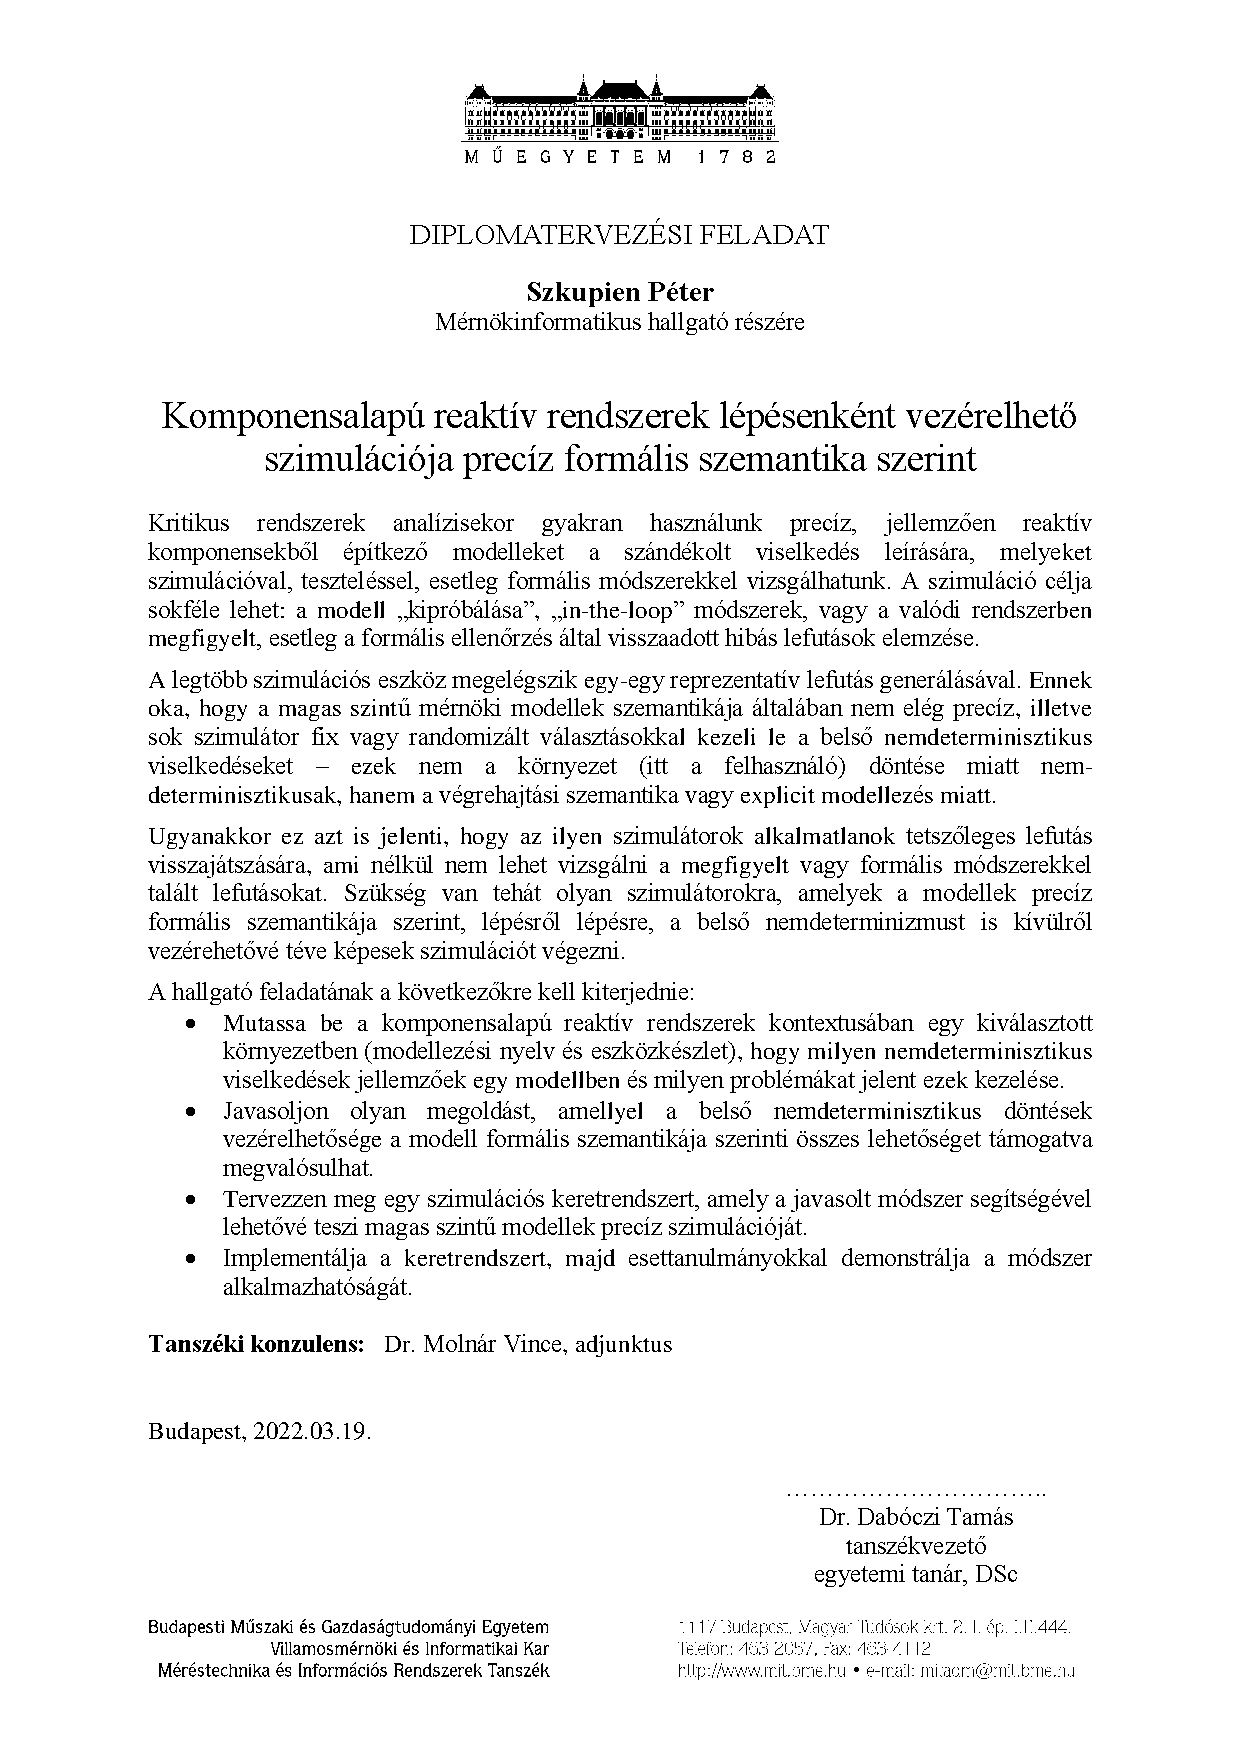
\includepdf[pages=-]{src/include/feladatkiiras.pdf}
     %Feladatkiírás

\hypersetup{pageanchor=false}
%--------------------------------------------------------------------------------------
%	The title page
%--------------------------------------------------------------------------------------
\begin{titlepage}
\begin{center}

\includegraphics[width=60mm,keepaspectratio]{figures/bme_logo.pdf}\\
\vspace{0.3cm}
\textbf{\bme}\\
\textmd{\vik}\\
\textmd{\viktanszek}\\[5cm]

\vspace{0.4cm}
{\huge \bfseries \vikcim}\\[0.8cm]
\vspace{0.5cm}
\textsc{\Large \vikdoktipus}\\[4cm]

{
	\renewcommand{\arraystretch}{0.85}
	\begin{tabular}{cc}
	 \makebox[7cm]{\emph{\keszitette}} & \makebox[7cm]{\emph{\konzulens}} \\ \noalign{\smallskip}
	 \makebox[7cm]{\szerzo} & \makebox[7cm]{\vikkonzulensA} \\
	  & \makebox[7cm]{\vikkonzulensB} \\
	  & \makebox[7cm]{\vikkonzulensC} \\
	\end{tabular}
}

\vfill
{\large \today}
\end{center}
\end{titlepage}
\hypersetup{pageanchor=false}

		   % Szakdolgozat/Diplomaterv címlap

\selectlanguage{magyar}
\pagenumbering{gobble}
%--------------------------------------------------------------------------------------
% Nyilatkozat
%--------------------------------------------------------------------------------------
\begin{center}
\large
\textbf{HALLGATÓI NYILATKOZAT}\\
\end{center}

Alulírott \emph{\vikszerzoVezeteknev{} \vikszerzoKeresztnev}, szigorló hallgató kijelentem, hogy ezt a \vikmunkatipusat{} meg nem engedett segítség nélkül, saját magam készítettem, csak a megadott forrásokat (szakirodalom, eszközök stb.) használtam fel. Minden olyan részt, melyet szó szerint, vagy azonos értelemben, de átfogalmazva más forrásból átvettem, egyértelműen, a forrás megadásával megjelöltem.

Hozzájárulok, hogy a jelen munkám alapadatait (szerző(k), cím, angol és magyar nyelvű tartalmi kivonat, készítés éve, konzulens(ek) neve) a BME VIK nyilvánosan hozzáférhető elektronikus formában, a munka teljes szövegét pedig az egyetem belső hálózatán keresztül (vagy autentikált felhasználók számára) közzétegye. Kijelentem, hogy a benyújtott munka és annak elektronikus verziója megegyezik. Dékáni engedéllyel titkosított diplomatervek esetén a dolgozat szövege csak 3 év eltelte után válik hozzáférhetővé.

\begin{flushleft}
\vspace*{1cm}
Budapest, \today
\end{flushleft}

\begin{flushright}
 \vspace*{1cm}
 \makebox[7cm]{\rule{6cm}{.4pt}}\\
 \makebox[7cm]{\emph{\vikszerzoVezeteknev{} \vikszerzoKeresztnev}}\\
 \makebox[7cm]{hallgató}
\end{flushright}
\thispagestyle{empty}

\vfill
\cleardoublepage

\selectthesislanguage
 %Hallgatói nyilatkozat

% Table of Contents
%~~~~~~~~~~~~~~~~~~~~~~~~~~~~~~~~~~~~~~~~~~~~~~~~~~~~~~~~~~~~~~~~~~~~~~~~~~~~~~~~~~~~~~
\tableofcontents\cleardoublepage


% Declaration and Abstract
%~~~~~~~~~~~~~~~~~~~~~~~~~~~~~~~~~~~~~~~~~~~~~~~~~~~~~~~~~~~~~~~~~~~~~~~~~~~~~~~~~~~~~~

\pagenumbering{roman}
\setcounter{page}{1}

\selecthungarian

%----------------------------------------------------------------------------
% Abstract in Hungarian
%----------------------------------------------------------------------------
\chapter*{Kivonat}\addcontentsline{toc}{chapter}{Kivonat}

A szoftveres megoldások folyamatosan terjednek az élet minden területén, amivel a biztonságkritikus szoftverrendszerek is egyre bonyolultabbá válnak. Ezen rendszerek minden körülmények között helyesen kell, hogy működjenek, ellenkező esetben a hibás működés katasztrofális következményekkel járna. Biztonságosságuk garantálására új fejlesztési elvek és módszerek terjedtek el, többek között a modellalapú rendszertervezés.

A modellalapú rendszertervezés alkalmazásához a mérnököknek magasszintű modellezési nyelvekre van szükségük, amelyek segítségével leírhatják a rendszerek különböző aspektusait. A rendszerek alapvető aspektusa a dinamikus viselkedés, amely leírására egyre népszerűbb a végrehajtható modellek használata. Ezek a modellek precíz formális szemantikával rendelkeznek, amelyet alacsonyszintű matematikai fogalmak segítségével definiálnak. A mérnökök által használt magasszintű modellek, és alacsony szinten definiált szemantikájuk közti absztrakciós szakadék megnehezíti a magasszintű modellek szemantikájának precíz megértését. Gyakori példa erre a magasszintű modellek atomi lépéseiben lévő belső nemdeterminizmus, amely csak a mögöttes alacsony szinten jelenik meg. Általános igény a mérnökök részéről, hogy a modelljeik szimulációja segítségével megfigyelhessék azok pontos viselkedését, ám a belső nemdeterminizmus a végrehajtások bizonyos részeit vezérelhetetlenné és megfigyelhetetlenné teszi, csökkentve ezzel a szimuláció precizitását.

Diplomatervemben bemutatok különböző absztrakciós szintű modellezési nyelveket, amelyeket komponensalapú reaktív rendszerek modellezésére használnak. A szemantikájukat alapul véve azonosítom a végrehajtásaik során előforduló lehetséges nemdeterminisztikus döntéseket, és bemutatom a saját algoritmusomat, amely a belső nemdeterminizmusokat külsővé alakítja. Erre építve megtervezek egy szimulációs keretrendszert, amely lehetővé teszi a felhasználó számára a szimuláció lépésenkénti vezérlését azáltal, hogy minden nemdeterminisztikus lépés vezérlését a felhasználóra bízza. Bemutatom a szimulátor különböző felhasználási módjait, amelyekhez megfelelő vezérlési mechanizmusokat is definiálok.

Az elméleti eredményeimet nyílt forráskódú eszközök (Gamma állapotgép-kompozíciós keretrendszer, Theta modellellenőrző keretrendszer) kiterjesztéseként implementáltam, amit tömören szintén bemutatok. Végül egy esettanulmányon keresztül elemzem a munkám eredményét, és demonstrálom annak használhatóságát.

\vfill
\selectenglish


%----------------------------------------------------------------------------
% Abstract in English
%----------------------------------------------------------------------------
\chapter*{Abstract}\addcontentsline{toc}{chapter}{Abstract}

Safety-critical software systems are becoming more and more complex with the continuous spreading of software solutions in all areas of life. These systems must operate correctly under all circumstances, otherwise, their fault would cause catastrophic consequences. Therefore, for guaranteeing safety, new development principles have been introduced, such as model-based systems engineering (MBSE).

To apply MBSE, engineers need high-level modeling languages for describing the different aspects of systems. One of the crucial aspects is the dynamic behavior, for which the application of executable models is spreading. These models have their precise formal semantics defined by low-level mathematical concepts. The abstraction gap between the high-level models used by engineers, and their semantics defined on a low level, makes it harder to understand the precise semantics of a high-level model. A common example of this is the internal non-determinism inside high-level atomic steps, which may only occur in the hidden low-level. It is a general need for engineers to be able to simulate their models, in order to observe their behavior precisely. Internal non-determinism makes some parts of the executions uncontrollable and unobservable, causing imprecise simulation.

In this thesis, I present some modeling languages with different abstraction levels which are used to model component-based reactive systems. Based on their semantics, I analyze the possible non-deterministic decisions of their execution and propose my own algorithm to make internal non-determinism external. Building on this, I design a simulation framework, which enables the user to control the simulation step-by-step, by making every non-deterministic decision explicit. I also identify different use cases, for which different simulation control mechanisms are presented.

I implemented my theoretical results as parts of open-source tools -- the Gamma Statechart Composition Framework, and the Theta Model Checking Framework -- which I also briefly present. Finally, the use of my work is discussed through a case study.

\vfill
\cleardoublepage

\selectthesislanguage

\newcounter{romanPage}
\setcounter{romanPage}{\value{page}}
\stepcounter{romanPage}    %Összefoglaló


% The main part of the thesis
%~~~~~~~~~~~~~~~~~~~~~~~~~~~~~~~~~~~~~~~~~~~~~~~~~~~~~~~~~~~~~~~~~~~~~~~~~~~~~~~~~~~~~~
\pagenumbering{arabic}

%import your own content
%----------------------------------------------------------------------------
\chapter{\bevezetes}
%----------------------------------------------------------------------------

With the continuous spreading of software solutions in all areas of life, software systems are becoming more and more complex. The increasing complexity requires new approaches to guarantee software quality, by using higher abstraction levels during design to reduce complexity. For this, engineers need convenient high-level modeling languages.

Models play a central role in the development process, especially in safety-critical domains (e.g., automotive, railway, aerospace industry) where engineering companies must use specific approaches in order to meet the corresponding standards. Model-based systems engineering (MBSE) is an actively spreading methodology for the development of complex, safety-critical systems~\cite{se2035}.

In MBSE, models are used to describe several different aspects of the designed system. A fundamental aspect is the behavior of the system, for which many formalisms are available for modeling. Due to the fact that complex systems usually have complex behavior, a high abstraction level is necessary for this aspect, too.

It is a common need for engineers to be able to observe the behavior of the designed system in design time to receive early feedback -- saving both working hours and money. To achieve this goal, a simulator for behavior models is necessary.

In order to precisely simulate behavioral models, having their formal semantics defined is crucial. Due to the high abstraction level of modeling languages used by engineers, the complexity of semantics is also high, making the simulation of such models challenging.

A common problem with complex semantics is non-determinism. Inside a single step of the high-level model, there may be non-deterministic decision points, enabling multiple different executions of a single step. Unfortunately, these inner decision points may remain hidden from the modeler, because executions with only inner differences can still lead the system to the same observable state. Furthermore, the different outputs can not be explained without the observation of the inner decisions.

In order to give full control to the engineers to be able to traverse any legal execution they want, the internal non-determinism of high-level atomic steps should be revealed and made explicit to the user. This could be achieved by breaking down the internally non-deterministic steps into smaller deterministic parts without changing the original semantics of the model.

In this thesis, I present the high-level statechart formalism for the design of component-based reactive systems, in which I present some examples of non-deterministic behavior. Statechart models can be transformed, e.g., into the lower-level extended symbolic transition system (XSTS) formalism~\cite{Gamma}, where non-determinism can still occur. I systematically analyze every source non-determinism in the XSTS formalism and propose an algorithm (called splitting) to make the internal non-determinism inside transitions external, enabling their observation.

Building on the splitting algorithm, I design a step-by-step controllable simulation framework for the precise simulation of split XSTS models. For guaranteed adherence to semantics, the simulation framework relies on an existing model checking infrastructure which is used for the semantics-critical calculation of successor states during the simulation.

This simulator enables the user to explicitly control every decision point during the simulation, regardless of whether it was originally internal or external. Based on the identified use cases, I also define and implement different control mechanisms for the simulator.

The rest of this thesis is structured as follows. In \autoref{background}, I give an overview of the theoretical background behind my work: formal methods, formal models, simulation, and the frameworks I contributed to. In \autoref{ch:reqs}, I define requirements on the simulation framework and design its high-level architecture. In \autoref{ch:splitting}, I formally present my XSTS transition splitting algorithm to make internal non-determinism external. In \autoref{ch:simulator}, I detail the simulation framework focusing on how it satisfies the requirements. In \autoref{example}, I present the use of the splitting algorithm and the simulation framework through a case study. Lastly, in \autoref{conclusion}, I summarize my work and present some future work.

\chapter{Background} \label{background}

In this chapter, I summarize the related background to this thesis. I briefly present formal methods and model checking (\autoref{sec:form-methods}), and formal models of different abstraction levels (\autoref{sec:form-models}). I also present the need for simulation (\autoref{sec:sim}) and the tools related to my work (\autoref{sec:tools}).

\section{Formal Methods}\label{sec:form-methods}

\textit{Formal methods} are precise approaches for the analysis of systems. They rely on mathematical logic, therefore they can be used only on mathematically precise \textit{formal models}. They are widely used for verification purposes in safety-critical domains (e.g., automotive, railway, and aerospace industries) where it is crucial to guarantee the safety of systems.

\subsection{Model Checking}

\textit{Model checking}~\cite{mc} is a formal method for the algorithmic analysis of the dynamic behavior of systems, checking whether a system satisfies a given requirement or not. The high-level overview of model checking is shown in \autoref{fig:mc}.

To apply model checking, three building blocks are required~\cite{IntroductionToModelChecking}:
\begin{itemize}
    \item \textit{Formal model}: A mathematically precise model of the behavior of the system is required, usually a \textit{transition system}~\cite{IntroductionToModelChecking}.
    \item \textit{Formal requirement}: The verifiable requirement should also be in a mathematically precise form, for which \textit{temporal logic}~\cite{tl} is appropriate.
    \item \textit{Algorithm}: Finally, an (effective) algorithm is required to decide whether the given formal model satisfies the given formal requirement or not. The output of the algorithm is a \textit{proof} or a \textit{counterexample}.
\end{itemize}

\begin{figure}[htbp]
\centering
\includesvg[inkscapelatex=false, width=0.9\textwidth, keepaspectratio]{figures/mc.svg}
\caption{Model checking.}
\label{fig:mc}
\end{figure}

Although with traditional \textit{testing} bugs can be found in systems, the correctness of a system can not be \textit{proved}. Model checking explores the entire state space of the system, making it possible to mathematically \textit{prove} that the system satisfies a certain requirement.

\section{Formal Models}\label{sec:form-models}

As systems -- especially safety-critical systems -- are becoming more complex, new development approaches, such as \textit{model-based systems engineering} (MBSE)~\cite{mbse}, have been introduced to handle complexity. In MBSE, models are the primary artifacts of the development process.~\cite{Seidewitz2003} To create these models, suitable modeling languages are required to model the different aspects of systems, e.g., structure or behavior.

In the case of \textit{behavioral models}, it is especially important to have precise formal semantics in order to be able to \textit{execute} them -- either by directly simulating them or by automatically transforming them into an executable formalism, e.g., program code.

\subsection{Component-Based Reactive Systems}

\textit{Component-based} development is a practical approach in the case of complex systems: engineers can compose such systems from reusable parts (\textit{components}) which are communicating with each other through well-defined interfaces.

\textit{Reactive} systems are interacting with their environment. These interactions are modeled as input and output events: input events coming from the environment can trigger internal behaviors (e.g., state change) of the system (i.e., the system \textit{reacts} to an event), while the system can react with output events to its environment. The possible interactions between the system and its environment can also be modeled with interfaces.

In the case of \textit{component-based reactive systems}, the components of the system can be modeled as \textit{state machines}~\cite{Gamma}. Informally, a state machine is a reactive component, because its behavior is modeled as \textit{transitions}, triggered by input events and generating output events.

\textit{State machines} are state-based models, focusing on the internal state of the system, and the transitions changing it. This modeling approach can be used at different abstraction levels. \textit{Finite state machine} (\autoref{ssec:fsm}) is a low-level mathematical, while \textit{Statechart} (\autoref{ssec:statechart}) is a high-level engineering formalism.

\subsection{Mathematical Finite State Machine}\label{ssec:fsm}

\textit{Finite state machine} is a mathematical formalism to model the state-based behavior of a system. Informally, it defines the possible states and state changes (\textit{transitions}) of a system. It can be either \textit{deterministic} or \textit{non-deterministic}, according to the number of possible transitions at a specific state, triggered by a specific input event.

\begin{definition}[Finite State Machine]\label{def:fsm}
    Formally, a deterministic finite state machine is a 5-tuple $SM = \langle S, s_0, I, O, T \rangle$ where:
    \begin{itemize}
        \item $S = \{ s_1, s_2, \ldots, s_n  \}$ is a finite set of \textit{states}.
        \item $s_0 \in S$ is the \textit{initial state}.
        \item $I = \{ i_1, i_2, \ldots, i_m \}$ is a finite set of \textit{input events} coming from the environment.
        \item $O = \{ o_1, o_2, \ldots, o_l \}$ is a finite set of \textit{output events} going to the environment. Note, that $I$ and $O$ are disjoint, i.e., $I \cap O = \emptyset$.
        \item $T: (I \times S) \mapsto (S \times O)$ is the (fully defined) \textit{transition function}, representing the reaction of the state machine to a specific input event in a specific state, i.e., the new state and the generated output event.
    \end{itemize}
\end{definition}

In Definition \ref{def:fsm}, I define a fully-defined deterministic finite state machine, i.e., which can take exactly one transition at every state, reacting to every input event. Note, that this does not mean, that the system must always change its state because a transition can lead the system to the same state as it was already in. The lack of the generated output event can be modeled with a special output event $\varepsilon$, i.e., a transition $T(i, s) = (s, \varepsilon)$ means that the system does not react to input event $i$ in state $s$.

Note, that the determinism of the state machine only means that the state machine itself is deterministic. Nevertheless, it can be used to model a system with a non-deterministic environment, by non-deterministically choosing the input events of the state machine.

\begin{example}[Finite State Machine]\label{ex:fsm}
    Consider a machine with two buttons, \emph{do} and \emph{reset}, which beeps after every third press of button \emph{do}, while the press of button \emph{reset} resets the counter. This machine can be modeled with the following deterministic finite state machine $SM = \langle S, s_0, I, O, T \rangle$:
    \begin{itemize}
        \item $S = \{ s_0, s_1, s_2  \}$ where $s_n$ represents the state where $n$ \emph{do} presses are counted since the last \emph{beep} or \emph{reset} press.
        \item $s_0 \in S$ is the \textit{initial state}.
        \item $I = \{ do, reset \}$ where the button presses are modeled as \textit{input events}.
        \item $O = \{ beep, \varepsilon \}$ where $beep$ models the beep of the machine as an \textit{output events}, and $\varepsilon$ models the lack of beep.
        \item $T =
        \begin{Bmatrix}
        (&do,& s_0,& s_1,& \varepsilon&),\\
        (&do,& s_1,& s_2,& \varepsilon&),\\
        (&do,& s_2,& s_0,& beep&),\\
        (&reset,& s_0,& s_0,& \varepsilon&),\\
        (&reset,& s_1,& s_0,& \varepsilon&),\\
        (&reset,& s_2,& s_0,& \varepsilon&)
        \end{Bmatrix}$
    \end{itemize}

    The transition function can be represented as a \emph{state-transition table}. Each cell represents the effect of the given input event in the given state as a pair of the next state and the output event.

    \begin{table}[htbp]
    \centering
    \begin{tabular}{|c||c|c|c|}
     \hline
     State/Input & $s_0$ & $s_1$ & $s_2$ \\
     \hline\hline
     $do$ & ($s_1$, $\varepsilon$) & ($s_2$, $\varepsilon$) & ($s_0$, $beep$) \\ 
     \hline
     $reset$ & ($s_0$, $\varepsilon$) & ($s_0$, $\varepsilon$) & ($s_0$, $\varepsilon$) \\
     \hline
    \end{tabular}
    %\caption{The state-transition table of finite state machine defined in \autoref{ex:fsm}.
    \label{tbl:stt}
    \end{table}

    The state machine can also be represented graphically as a graph. The nodes represent the states, while the edges represent the transitions. An edge with label $i / o$ represents a transition leading the system from the state represented by the source node to the state represented by the target node, triggered by input event $i$, producing output event $o$.

    \begin{figure}[htbp]
    \centering
    \includesvg[inkscapelatex=false, width=0.5\textwidth, keepaspectratio]{figures/fsm.svg}
    \caption{Graphical representation of the example finite state machine.}
    \label{fig:fsm}
    \end{figure}
    
\end{example}

\subsection{High-Level Statechart}\label{ssec:statechart}

The \textit{statechart} formalism is a popular tool to model the behavior of state-based reactive systems in a higher abstraction level~\cite{Harel}. It relies on the mathematical \textit{finite state machine} formalism but it is more expressive, making the formalism usable in everyday engineering work.

In general, the statechart formalism extends the finite state machine formalism with the following:
\begin{itemize}
    \item \textit{Hierarchically nested states}: The internal behavior of a state (\textit{superstate}) can be modeled with an inner statechart (\textit{substates}). The inner statechart operates in the context of the superstate. When the superstate is activated, its initial inner state activates, too. When the superstate is deactivated, its whole inner statechart deactivates.
    \item \textit{Orthogonal regions}: The internal behavior of a state can be modeled with several statecharts (\textit{regions}), running independently.
    \item \textit{Entry and exit actions}: Like in the case of transitions, \textit{entry} and \textit{exit} actions can be defined for states. These actions are triggered when the state is activated or deactivated, respectively.
\end{itemize}

\begin{example}[Statechart]\label{ex:sch}
    Consider the extension of the finite state machine defined in Example \ref{ex:fsm}. A new input event \emph{switch} is introduced to switch the whole machine on/off. When the machine is switched on/off, it beeps. When the machine is turned on, it beeps when the reset button is pressed first since the machine is turned on.

    It serves as an example for all of the three new features of the statechart formalism. The initial \emph{Off} state defines an entry and exit action for beeping. The hierarchical \emph{On} state contains two orthogonal regions which are independently responsible for counting the \emph{do} and \emph{reset} events.

    The graphical representation of this statechart is shown below.

    \begin{figure}[htbp]
    \centering
    \includesvg[inkscapelatex=false, width=0.8\textwidth, keepaspectratio]{figures/sch.svg}
    \caption{Graphical representation of the example statechart.}
    \label{fig:sch}
    \end{figure}
    
\end{example}

The statechart formalism can be further extended, e.g. with \textit{variables} and \textit{guards}. Guards on transitions are logical expressions over variables, and a transition can not be fired if its guard evaluates to false.

The informally introduced high-level formalism has several concrete definitions in different modeling languages such as the general-purpose \textit{Unified Modeling Language}(UML)~\cite{uml} and \textit{Systems Modeling Language} (SysML)~\cite{sysml} developed by the \textit{Object Management Group} (OMG), though these formalisms often lack precise formal semantics~\cite{Elekes2022}.

\subsubsection{Non-Determinism}

The execution of a statechart can be non-deterministic due to several reasons. In general, we distinguish two types of non-determinism: \textit{internal} and \textit{external}.

\paragraph{Internal non-determinism.} A single step of a statechart can contain non-deterministic decision point(s). This means, that in a specific state configuration, with a specific input event, the statechart can behave in different ways. Due to the fact, that the environment can only interact with the statechart with input events (i.e., the statechart itself is a \textit{black box} in terms of control), internal non-determinism makes the behavior of the system uncontrollable, causing problems in several use cases, e.g., precise simulation.

The systematic analysis of (internal) non-determinism in statechart semantics is beyond the scope of this work, here I only highlight some examples to underline its necessity.

\begin{itemize}
    \item \textit{Multiple fireable transitions}: In real-life engineering work, especially with the growing complexity of state hierarchies and guard expressions, statecharts are usually not deterministic and fully defined. This means, that in a specific state configuration, an input event may trigger multiple transitions. Although state machine semantics usually define some rules to select the transition to fire, in some cases neither of these rules defines the \textit{exact} transition(s) to fire, i.e., the choice from the firable transitions remains non-deterministic.
    \item \textit{Orthogonal regions}: The execution of orthogonal regions is independent, meaning that there is no guarantee on the order of their steps. As a result, the exact ordering is non-deterministic.
    \item \textit{Composition}: Individual statecharts usually serve as components of a more complex system. In this case, the composition of the statecharts may not define their exact execution order, causing non-determinism, too.
    %\item \textit{Environment}: The environment of statecharts is usually modeled using non-determinism to cover the possible inputs. This kind of non-determinism is intentional, making it necessary to select the actual environment behavior during execution explicitly.
\end{itemize}

\paragraph{External non-determinism.} An obvious source of non-determinism during execution is the behavior of the \textit{environment}, i.e., the input events sent to the statechart. This is called external non-determinism, and does not cause problems like internal non-determinism. External non-determinism is observable and controllable, e.g., during simulation, it is typically handled by the user of the simulator by ``impersonating`` the environment, i.e., choosing the next event to send (and its parameters, if any).


\subsection{Extended Symbolic Transition System}\label{ssec:xsts}

Extended Symbolic Transition System (XSTS)~\cite{XSTS} is a suitable low-level formalism to describe higher-level (reactive) systems, such as statecharts. Informally, an XSTS model describes variables and transition sets, and in every step a non-deterministically selected atomic transition fires from the appropriate transition set. In this thesis, I introduce XSTS based on my previous work~\cite{xsts-split}.

\begin{definition}[Extended Symbolic Transition System]
Formally, an XSTS model is a 4-tuple $XSTS = \langle V, Tr, In, En \rangle$ where:
\begin{itemize}
    \item $V = \{ v_1, v_2, \ldots, v_n  \}$ is a set of \textit{variables} with domains $D_{v_1}, D_{v_2}, \ldots, D_{v_n}$, e.g. \emph{integer}, \emph{bool}, or \emph{enum}. An \emph{enum} domain is just syntax sugar, a set of \emph{literals} which are different values with a textual representation.
    \item A state of the system is $s \in S \subseteq D_{v_1} \times D_{v_2} \times \cdots \times D_{v_n}$, which can be regarded as a value assignment: $s(v) \in D_v$ for every variable $v \in V$.
    \item $Tr \subseteq S \times S$ is the \textit{internal transition relation}, describing the behaviour of the system itself;
    \item $In \subseteq S \times S$ is the \textit{initial transition relation}, describing the initialization of the system, which is executed only once at the beginning of the execution;
    \item $En \subseteq S \times S$ is the \textit{environmental transition relation}, describing the environment which the system is interacting with;
    \item Both $Tr$, $In$, and $En$ may be defined as a union of individual transitions that the system can take. Abusing the notation, we will denote these transitions as $t \in Tr$ which actually means that $t \subseteq S \times S$ as a transition relation is a subset of $Tr$.
\end{itemize}
\end{definition}

A \textit{concrete state} of the system is $c \in C = D_{v_1} \times D_{v_2} \times \cdots \times D_{v_n}$, which is a value assignment $c: v \mapsto c(v) \in D_v$ for every variable $v \in V$. A concrete state $c$ can also be described with a logical formula $\varphi = (v_1 = c(v_1) \wedge \cdots \wedge v_n = c(v_n))$ where $\mathrm{var}(\varphi) = V$.
%A concrete state $c$ can also be described with a logical formula $\varphi$ where $var(\varphi) \subseteq V$ or $var(\varphi) = V$ if $\top \in D_v$ for every $v \in V$ where $v = \top$ means there is no restriction on the value of $v$ so it can be anything from $D_v$.

%= 2^{D_{v_1}} \times 2^{D_{v_2}} \times \cdots \times 2^{D_{v_n}}$
An \textit{abstract state} of the system $s \in S = 2^C$ may cover more concrete states $s = \{ c_1, \ldots, c_m \}$. We use the notation $0 \leq |s| \leq 2^{|C|}$ for the number of concrete states covered by abstract state $s$. Like in the case of concrete states, the notation $s(v) = x$ where $x \in D_v$ means that $c(v) = x$ in every concrete state $c \in s$ covered by $s$.
%If there is no restriction on variable $v$, i.e. it can have any value from $D_v$, we use the notation $s(v) = \top$.
The logical formula of an abstract state is $\varphi = ((v_1 = c_1(v_1) \wedge \cdots \wedge v_n = c_1(v_n)) \vee \cdots \vee (v_1 = c_m(v_1) \wedge \cdots \wedge v_n = c_m(v_n)))$ where $\mathrm{var}(\varphi) = V$, and it covers exactly $m$ (maybe infinite) concrete states.

Note, that every concrete state $c$ is also an abstract state $s$ covering only 1 concrete state $c$, so $|c| = |s| = 1$. Thus, without the loss of generality, we use abstract states in the following even without explicitly stating that a state is abstract.

Each transition relation $T \in \{ Tr, In, En \}$ is a set of transitions $t$ where a transition leads the system from a state $s$ to a successor states $s'$: $T \subseteq \{ t=(s, s') \in S \times S \}$.

Every domain $D$ has an initial value $IV(D) \in D$ e.g., $IV(\textit{bool}) = \textit{false}$, $IV(\textit{integer}) = 0$. Every variable $v$ can have a custom initial value $IV(v) \in D_v$ but it is not necessary, because its domain $D_v$ always has one. The only (concrete) \emph{initial state} $s_0$ is given as the \emph{initial value} for each variable $v$: $s_0(v) = IV(v)$ if $IV(v)$ exists, otherwise $s_0(v) = IV(D_v)$. The execution of the system starts with assigning the initial value $s_0(v)$ to every variable $v \in V$.

From the initial state $s_0$, $In$ is executed exactly once. Then, $En$ and $Tr$ are executed in alternation. In state $s$, the execution of a transition relation $T$ (being either of the transition relations) means the execution of exactly one non-deterministically selected $t \in T$ transition. Transition $t$ is enabled if $t(s) \neq \emptyset$. If a transition is not enabled, it can not be executed. If $\forall t \in T: t(s) = \emptyset$, transition relation $T$ can not be executed in state $s$, and therefore $s$ is a deadlock. In addition to the non-deterministic selection, transitions may be non-deterministic internally, therefore even in the case of a concrete state $c$, $t(c) = \{c^\prime_1, \ldots, c^\prime_k\}$ may yield a set of successor concrete states. In other words, in the case of a general transition $t=(s, s^\prime)$, there is no restriction on the relation between $|s|$ and $|s^\prime|$.

\subsubsection{XSTS Operations}\label{ssec:xsts-ops}
Transitions are described as $op \in Ops$ \textit{operations}, which may be atomic or composite operations. The semantics of transitions are defined through the semantics of operations, which is, in turn, the definition of $op$ as a relation over $S \times S$. For a precise description, refer to~\cite{XSTS} -- for this work, an informal definition is sufficient.

XSTS defines the following \emph{basic operations} which lead the system from state $s$ to successor state $s^\prime$:
    \begin{itemize}
        \item \textit{Assignments}: An assignment of form $v := \varphi$ with $v \in V$ and $\varphi$ as an expression of the same type $D_v$ means that $\varphi$ is assigned to $v$ in the successor state $s^\prime$ and all other variables keep their value. Formally, $s^\prime = \bigcup c^\prime$, where $c^\prime(v) = \varphi \wedge c^\prime(v^\prime) = c(v^\prime)$ for every $v^\prime \neq v \in V$ and every $c \in s$. Therefore, the number of concrete states covered by $s^\prime$ is less than or equal to the number of concrete states covered by $s$: $|s^\prime| \leq |s|$.
        \item \textit{Assumptions}: An assumption of form $[\psi]$ with $\psi$ as a Boolean expression over the variables ($\mathrm{var}(\psi) \subseteq V$) checks condition $\psi$ without modifying any variable and can only be executed if $\psi$ evaluates to \textit{true} over the current state $s$, i.e., over at least one concrete state $c \in s$. In this case, the successor state $s^\prime$ covers the concrete states $c \in s$ covered by the original state $s$ where $\psi$ evaluates to \textit{true}, therefore $|s^\prime| \leq |s|$. Otherwise, i.e., when $\psi$ evaluates to \textit{false} over every concrete state $c \in s$, the set of successor states is the empty set $\emptyset$, and $|s^\prime| = 0$.
        \item \textit{Havocs}: A havoc of form $\havoc(v)$ with $v \in V$ means a non-deterministic assignment to variable $v$, i.e., after execution, the value of $v$ can be anything from $D_v$ and all other variables keep their value. Formally, $s^\prime = \bigcup_{c \in s} \{ c^\prime_1, \ldots, c^\prime_{|D_v|} \}$, where $c^\prime_i(v) = D_{v_i} \wedge c^\prime_i(v^\prime) = c_i(v^\prime)$ for every $v^\prime \neq v \in V$ where $D_v = \{ v_1, \ldots, v_{|D_v|} \}$. Therefore, $|s^\prime| \geq |s|$.
        \item \textit{Local variables}: A local variable can be declared as an operation of form $\mathit{var}\ v_{\mathit{\mathrm{loc}}} : \mathit{type} :=\varphi$.\footnote{The default value of the type is used as an initializer unless explicitly specified by the modeler.} A local variable can only be accessed in its \textit{scope} which is its direct container composite operation. Technically, the declaration of a local variable $v_{\mathrm{loc}}$ adds it to $V$ and assigns its initial value $\varphi$ to $v_{\mathrm{loc}}$ while the end of every scope removes every local variable declared in it from $V$. Thus, local variables increase the state space \textit{only} inside their container transitions. Due to the atomicity of transitions, local variables do not modify the state space of the system itself. Formally, $V^\prime = V \cup \{ v_{\mathrm{loc}} \}$, $s^\prime(v_{\mathrm{loc}}) = \varphi$, $s^\prime(v) = s(v)$ for every $v \in V$, and $|s^\prime| = |s|$.
    \end{itemize}
\emph{Composite operations} contain other operations but their execution is still atomic. Practically, this means that the contained operations are defined over transient states and the composite operation determines which one(s) will be the (stable) result of the composite operation. XSTS defines the following composite operations:
    \begin{itemize}
        \item \textit{Sequences}: A sequence of form $op_1, \ldots, op_n$ is composed of operations $op_1, \ldots, op_n$ with $op_i \in Ops$ executed sequentially, each applied on every successor state of the previous one (if any). The successor state after executing the sequence is the result of the last operation.
        Each operation $op_{i+1}=(s_{i+1}, s^\prime_{i+1})=(s^\prime_{i}, s^\prime_{i+1})$ works on the result of $op_i=(s_{i}, s^\prime_{i})$, so $s^\prime_{i} = s_{i+1}$. Thus, the transition of the sequence itself is $(s_{1}, s^\prime_{n})$ but it can be executed only if $s^\prime_{i} \neq \emptyset$ for every $1 \leq i \leq n$, i.e. all assumptions are satisfied.
        
        \item \textit{Choices}: A choice of form $op_1$ or $\ldots$ or $op_n$ means a non-deterministic choice between operations (branches) $op_1, \ldots, op_n$ with $op_i \in Ops$. This means that exactly one executable branch $op_i$ will be executed. A branch $op_i = (s_{i}, s^\prime_{i})$ can not be executed if $s^\prime_{i} = \emptyset$, i.e. an assumption does not hold in the branch. If there are both executable and non-executable branches, an executable one must be executed. If all branches are non-executable ($s^\prime_{i} = \emptyset$ for every $1 \leq i \leq n$), the choice itself is also non-executable, so its successor state is $\emptyset$. Generally, the set of successor states is the union of the results of any branch $\cup_{i=0}^{n} s^\prime_{i}$.
        
        \item \textit{Conditionals}: A conditional of form $(\psi)\ ?\ op_{\mathrm{then}}\ :\ op_{\mathrm{else}}$ with $\psi$ as a Boolean expression over the variables ($\mathrm{var}(\psi) \subseteq V$) checks condition $\psi$, and executes $op_{\mathrm{then}} = (s_{\mathrm{then}}, s^\prime_{\mathrm{then}})$ if $\psi$ evaluated to true, otherwise $op_{\mathrm{else}} = (s_{\mathrm{else}}, s^\prime_{\mathrm{else}})$ ($op_{\mathrm{else}}$ can be empty, i.e. a 0-long sequence, when $s_{\mathrm{else}} = s^\prime_{\mathrm{else}}$). The sccessor state of the conditional $(s, s^\prime)$ is $s^\prime = s^\prime_{\mathrm{then}}$ if $\psi$ is true over the variable values of $s$, otherwise $s^\prime = s^\prime_{\mathrm{else}}$.
        
        \item \textit{Parallels}: A parallel of form $op_1$ || $\ldots$ || $op_n$ means the parallel execution of operations (branches) $op_1, \ldots, op_n$ with $op_i \in Ops$. The parallel execution means that one substep of the parallel execution is a substep of a non-deterministically selected branch, which has not finished its execution. The parallel action finishes when all of its branches have finished.
    \end{itemize}
    
Note that assumptions may cause any composite operation to yield an empty set as the set of successor states. This allows us to use the \emph{choice} operation as a guarded branching operator, ruling out branches where an assumption fails by yielding an empty set as the result of that branch.

In this work, we make the following assumptions, which can be easily guaranteed by simple pre-processing.
\begin{enumerate}
    \item The operation of transitions and non-sequence composite actions must be composite actions. Thus, single basic operations will be treated as 1-long sequences.
    \item We assume that there are no sequences directly inside sequences.
\end{enumerate}
These restrictions help the clarity and consistency of local variable scopes without the loss of generality.

\subsubsection{Transition Granularity in XSTS Models} \label{ssec:xsts-gran}

The execution of a transition relation means a non-deterministic choice over the transitions of the relation. In addition, transitions can also be non-deterministic internally. After executing transition $t=(s, s^\prime)$ from state $s$, we can only observe state $s^\prime$ but the possible internal non-determinism of $t$ remains invisible. To make the execution of the system fully explainable we have to make every non-deterministic choice observable. This can be achieved by making internal non-determinism external by splitting the transitions into smaller ones.

The basics of this splitting approach are presented in my previous work~\cite{xsts-split}. In \autoref{ch:splitting}, I extend and formalize the splitting model transformation in order to make the executions fully explainable without changing the original semantics of the XSTS model.

\section{Simulation}\label{sec:sim}

In everyday engineering work, it is useful if engineers can observe the behavior of the designed systems in an early stage of development. These observations can provide early feedback about different aspects of the system, reducing the cost of the whole development process. Due to this need, simulators are required which can simulate high-level engineering models.

With the growing complexity of the designed systems, the abstraction level of engineering models is also increasing. During the simulation of high-level models, the simulator repeatedly calculates the successor states of the system in every simulation step. At the core of the simulator, this calculation can be broken down into low-level mathematical operations. It is a challenge for the simulator to fill the abstraction gap between the actual calculations and the high-level steps.

An example of this challenge is the internal non-determinism of high-level simulation steps. An atomic high-level step may contain hidden decision points at a lower level, e.g. an atomic step of a statechart may contain a decision point if multiple transitions are fireable. For precise simulation, it is important to make these internal decision points explicit to the user, in order to give them a better understanding of the possible behaviors of the designed system.

In the case of statecharts, most simulation tools do not enable the user to simulate every possible behavior, e.g., they do not make it possible to select the exact execution order of parallel regions.

\section{Related Tools}\label{sec:tools}

In my work, I extended two open source frameworks -- the Gamma Statechart Composition Framework (\autoref{ssec:gamma}), and the Theta Model Checking Framework (\autoref{ssec:theta}) -- both developed at the Critical Systems Research Group\footnote{\url{https://ftsrg.mit.bme.hu/en/}} of the Department of Measurement and Information Systems, Budapest University of Technology and Economics.

\subsection{Gamma Statechart Composition Framework}\label{ssec:gamma}

The \textit{Gamma Statechart Composition Framework}\footnote{\url{https://inf.mit.bme.hu/en/gamma} and \url{https://github.com/ftsrg/gamma}}~\cite{Gamma} is an Eclipse-based framework for the model-based design and formal analysis of component-based reactive systems. Gamma has its own modeling languages for the definition of individual \textit{statecharts} and their \textit{composition}. For such concepts, Gamma defines their precise formal semantics, making the use of formal methods possible.

Defining models in the Gamma Statechart Language is not the only way to use Gamma. For real-life usability, Gamma supports the integration of high-level engineering models (e.g., Yakindu and SysML statecharts) by providing X-to-Gamma model transformations. This architecture also makes the framework easily extendable with the support of further modeling languages.

Gamma statecharts support the common features of engineering-level statecharts, e.g., the modeling of \textit{variables} with different \textit{domains}, state refinement, and concurrent regions.

Once Gamma models are available (regardless of their origin), the framework provides numerous features.

\begin{itemize}
    \item \textit{Visualization}: Gamma can visualize the designed statecharts and the composite systems in graphical diagrams using PlantUML\footnote{\url{https://plantuml.com/}}.
    \item \textit{Validation}: Gamma provides several validation rules to statically analyze the models in design time, presenting warnings or errors to the user. These give valuable early feedback to the modeler about the possible errors of the modeled system.
    \item \textit{Formal verification}: Gamma can apply formal verification on models. It provides a custom language to define the verifiable requirements (as temporal logic formulas), and transforms the models and the requirements into the input formalism of the selected formal verification backend. Currently, it supports UPPAAL~\cite{uppaal} (extended timed automaton formalism), Theta~\cite{Theta} (extended symbolic transition system formalism), and SPIN~\cite{spin} (Promela formalism) as formal verification backends. It also back-annotates the low-level verification result to the Gamma-level models.
    \item \textit{Code generation}: Gamma can transform composite models into Java source code, keeping its component-based structure. For every Gamma-level interface, component, and system a separate Java interface or class is generated, respectively.
    \item \textit{Test generation}: Gamma can generate test cases to fulfill different coverage criteria (e.g., state coverage, transition coverage). The resulting test cases are presented at the Gamma level (in the Gamma Test Language) and can also be transformed into Java code, as JUnit tests.
\end{itemize}

The model transformation chains and languages of the Gamma framework are shown in \autoref{fig:gamma}.

\begin{figure}[htbp]
\centering
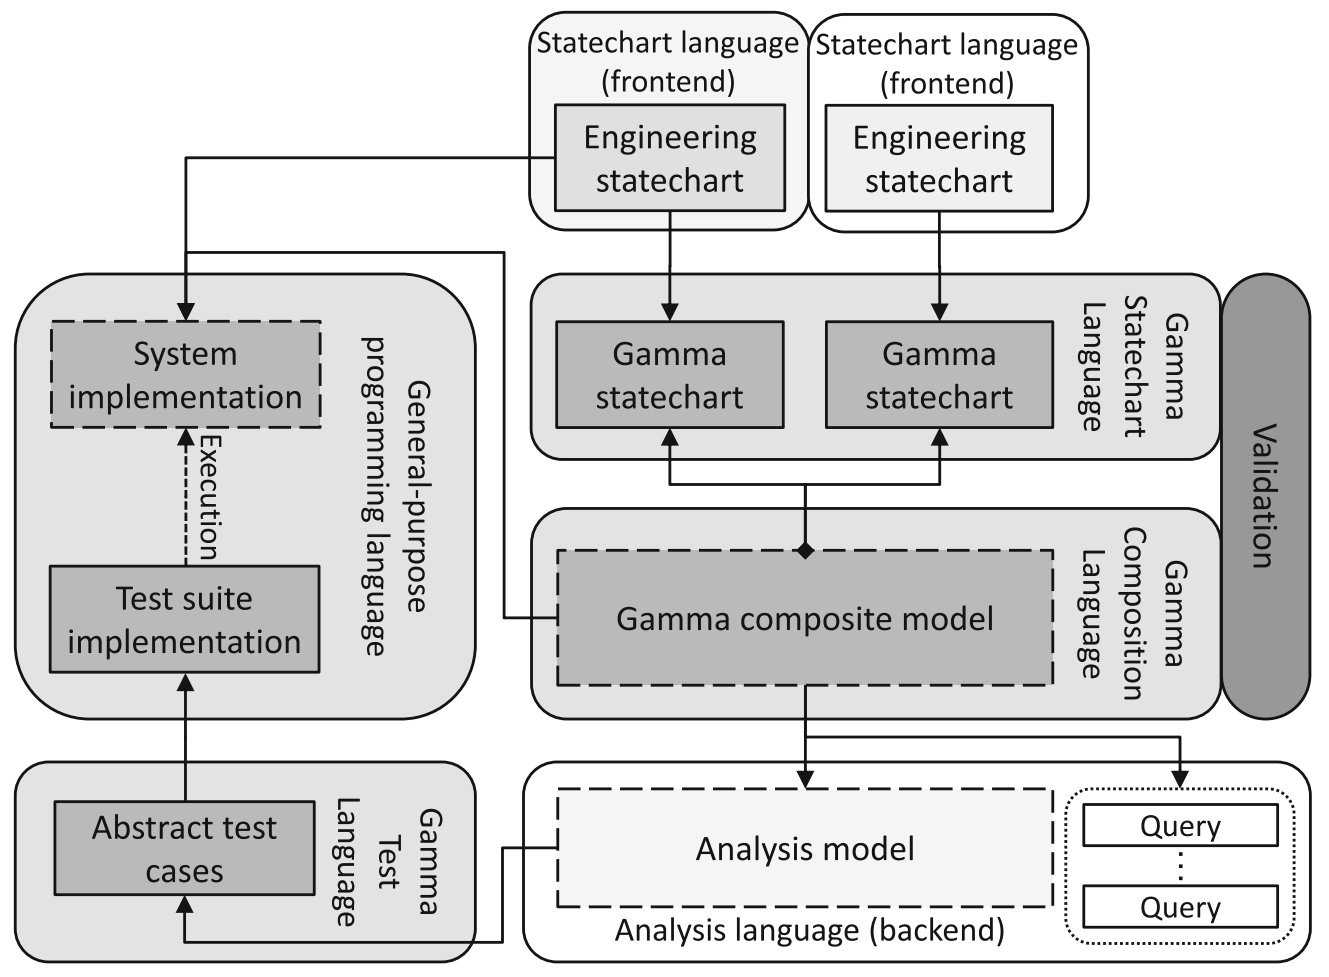
\includegraphics[width=0.8\textwidth, keepaspectratio]{figures/gamma.png}
\caption{The functionalities of the Gamma framework~\cite{Graics2020}.}
\label{fig:gamma}
\end{figure}

\subsection{Theta Model Checking Framework}\label{ssec:theta}

The Theta Model Checking Framework\footnote{\url{https://inf.mit.bme.hu/en/theta} and \url{https://github.com/ftsrg/theta}}~\cite{Theta} is a generic, modular, and configurable model checking framework. The architecture of Theta is shown in \autoref{fig:theta}.

\begin{figure}[htbp]
\centering
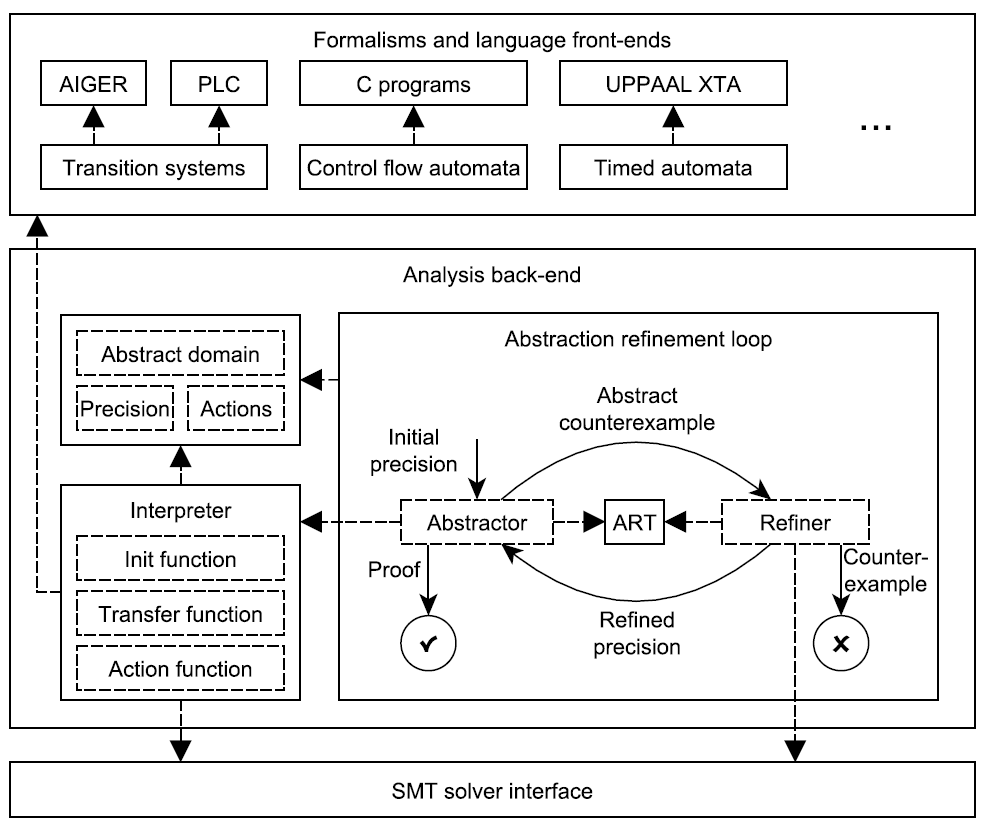
\includegraphics[width=0.8\textwidth, keepaspectratio]{figures/theta.png}
\caption{The architecture of the Theta framework~\cite{Theta}.}
\label{fig:theta}
\end{figure}

Theta can be divided into four main layers.

\begin{itemize}
    \item \textit{Formalisms}: Theta can handle multiple formalisms as input, such as \textit{timed automata}, \textit{control flow automata}, and \textit{transition systems}. Due to its modular architecture, further formalisms can be integrated. Every input model is transformed into a common inner abstract state space representation, regardless of the original input formalism. In this work, I focus on the \textit{Extended Symbolic Transition System} (XSTS)~\cite{XSTS} formalism as the input of Theta.
    \item \textit{Analysis back-end}: The analysis back-end provides the verification algorithms themselves. It contains formalism-specific \textit{interpreters} providing a common interface towards the algorithms by defining three functions: the \textit{init function} calculates the initial abstract states of the system, the \textit{transfer function} calculates the successor states of a given state, and the \textit{action function} calculates the available actions in a given abstract state. The verification algorithms usually use abstraction for which various \textit{abstract domains} are defined.
    \item \textit{SMT solver interface}: Many components rely on \textit{satisfiability modulo theories}~\cite{smt} (SMT) solvers for which a general interface is provided by Theta. It enables the use of different SMT solvers, and currently, it fully supports the Z3\footnote{\url{https://github.com/Z3Prover/z3}} solver developed by Microsoft.
    \item \textit{Tools}: Theta provides simple command-line applications which are responsible for reading the input and then instantiating and calling the algorithm specified by the arguments.
\end{itemize}

The analysis is done by the \textit{counterexample-guided abstraction refinement} (CEGAR) loop in the analysis back-end, Its central data structure is the \textit{abstract reachability graph}~\cite{theta-arg} (ARG) or \textit{abstract reachability tree} (ART). Its nodes represent abstract states, and its edges are labeled with actions. The ARG is modified by the two main parts of the loop, the \textit{abstractor} and the \textit{refiner}.

The initial ARG is constructed by the abstractor, based on the initial precision which comes from the selected algorithm and the formalism-specific interpreter. If there is no counterexample in the ARG, it \textit{proves} the correctness of the model. Otherwise, if an abstract counterexample exists, the refiner checks its feasibility. If the abstract counterexample is feasible, i.e., real, the model is incorrect, and the counterexample is returned. Otherwise, the refiner refines the abstraction of the ARG to eliminate that spurious counterexample.

%own chapters...
\chapter{Requirements on the Simulation Framework} \label{ch:reqs}

In this chapter, I declare the main requirements on the simulation framework. The requirements cover semantics (\autoref{sec:req-semantics}), variable values (\autoref{sec:req-varvals}), back-annotation (\autoref{sec:req-backannotate}), non-determinism (\autoref{sec:req-nondet}), control (\autoref{sec:req-control}), and observation (\autoref{sec:req-observ}). I analyze the requirements, and as a result, present some design decisions and the high-level architecture of the simulation framework (\autoref{sec:sim-architecture}).

The requirement diagram of the simulator is shown in \autoref{fig:reqs}.

\begin{figure}[htbp]
	\centering
	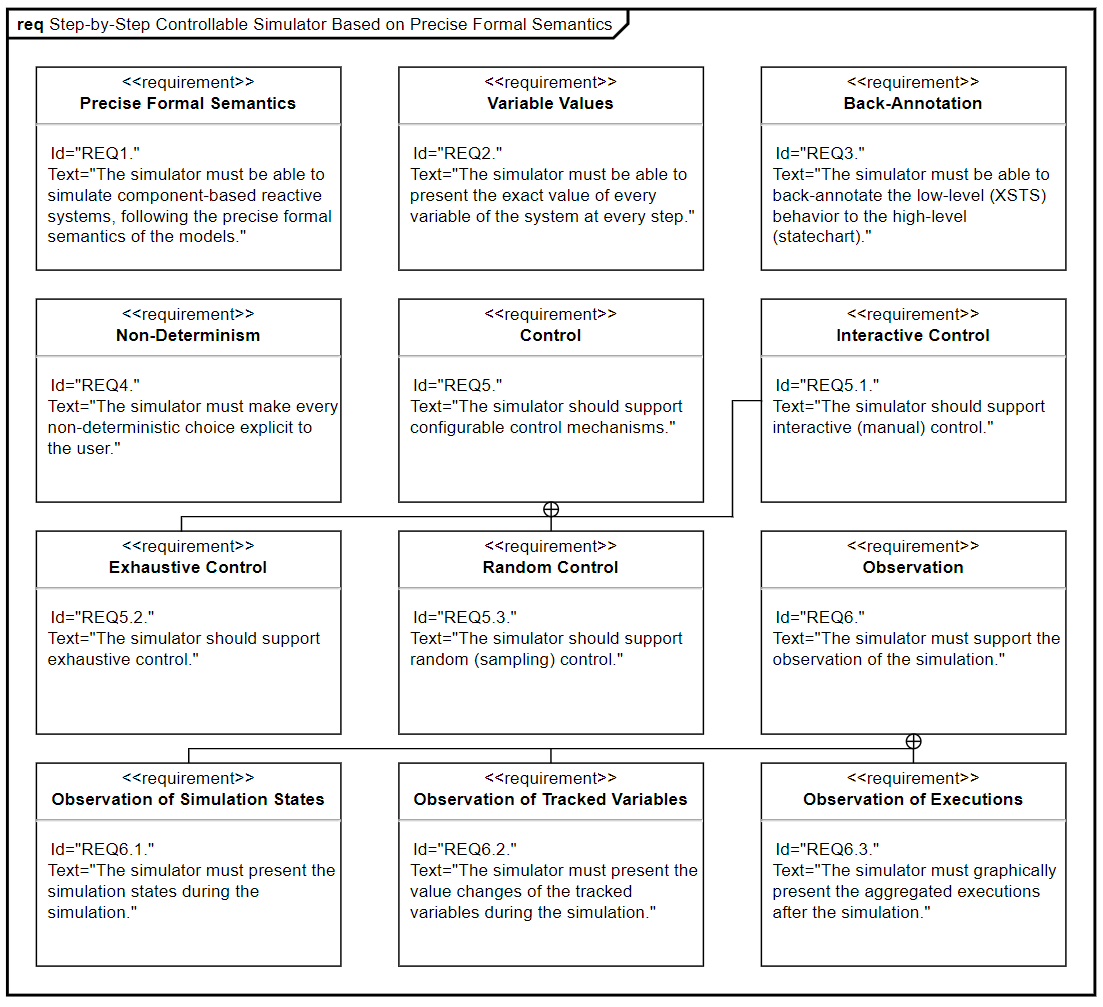
\includegraphics[width=\textwidth, keepaspectratio]{figures/reqs.png}
	\caption{Requirement Diagram of the simulator.}
	\label{fig:reqs}
\end{figure}

\section{Precise Formal Semantics}\label{sec:req-semantics}

\paragraph{REQ1.} \textit{The simulator must be able to simulate component-based reactive systems, following the precise formal semantics of the models.}

Component-based reactive systems can be modeled with Gamma statecharts. Although Gamma statecharts have precise formal semantics, their direct simulation would be hard due to their complexity and high-abstraction level. For formal verification purposes, Gamma provides a semantics-preserving Gamma-to-XSTS model transformation which can be reused for simulation, too. The simulation of XSTS models is easier, due to their lower abstraction level.

In order to follow the exact semantics of XSTS models during simulation, I decided to reuse the model checker infrastructure of Theta, so exactly the same code calculates e.g., the successor states of a state during the simulation and formal verification. With this approach, I can save a lot of unnecessary work and avoid redundant code bases, resulting in easier maintainable software components.

\section{Variable Values}\label{sec:req-varvals}

\paragraph{REQ2.} \textit{The simulator must be able to present the exact value of every variable of the system at every step.}

An important use case of the simulation of behavioral models is that engineers can try out the models they designed. The more details a simulator can give to its user, the more useful it is. It is crucial to always be able to present the simulation state to the user, which, in the case of XSTS models, consists of the exact value of every variable of the system including variables encoding the state of execution (control variables).

The model checking infrastructure of Theta supports the usage of abstraction-based algorithms, such as counterexample-guided abstraction refinement (CEGAR). Abstraction improves the efficiency of model checking, which leads to the support of more complex models. In the case of simulation, efficiency is not a key requirement, so instead of any kind of abstraction, the simulator makes the underlying model checker infrastructure explicitly track the value of every variable.

\section{Back-Annotation}\label{sec:req-backannotate}

\paragraph{REQ3.} \textit{The simulator must be able to back-annotate the low-level (XSTS) behavior to the high-level (statechart).}

Although the simulator simulates the statecharts by generating a semantics-preserving XSTS model from them and simulating the XSTS model itself, it is expected to observe the behavior of the original statechart model, not the XSTS model. To fill the abstraction gap, proper back-annotation could be provided to map every change in the low-level model state to a higher-level behavior, but this is beyond the scope of this work.

Instead, the back-annotation in my work relies on the log mechanism of Gamma. In the high-level statecharts, explicit \textit{log} statements can be defined with a custom string literal. During the Gamma-to-XSTS model transformation, the log statements of every component are transformed into lower-level model elements.

\begin{itemize}
    \item For every \textit{component type}, an XSTS enum type is created, with the same literals as the literals used in the log statements of the component, and a default literal $\mathit{None}$.
    \item For every \textit{component instance}, an XSTS variable is created, with the enum domain corresponding to its component type, and the default value $\mathit{None}$.
    \item For every \textit{log statement}, an XSTS assignment is created, which assigns the enum literal corresponding to the log literal, to the variable corresponding to the component instance. Then, the variable needs to be reset so the default value $\mathit{None}$ is assigned to it.
\end{itemize}

During the simulation of the low-level XSTS model, the value changes of these log variables can be observed to follow the execution of the high-level statechart models.

\begin{example}[Transformation of log statements]
    Consider a component type $T$, and component instances $a$ and $b$ of type $T$. In $T$ (e.g., in the high-level statechart transitions), log statements are defined with string literals $\mathit{log1}$ and $\mathit{log2}$.

    During the Gamma-to-XSTS model transformation, the following log-related model elements are created:
    \begin{itemize}
        \item For component type $T$, an XSTS enum type $D_{\mathrm{log}_T}$ is created with literals $\mathit{None}$, $\mathit{log1}$, and $\mathit{log2}$.
        \item For component instances $a$ and $b$, XSTS variables $\mathit{log}_a$ and $\mathit{log}_b$ are created, with the same domain $D_{\mathrm{log}_T}$. The initial value of every log variable is the default log literal $\mathit{None}$.
        \item E.g., in the case of component instance $a$, the log statement with string literal $\mathit{log1}$ is transformed to XSTS assignments $\mathit{log}_a := \mathit{log1}$, and $\mathit{log}_a := \mathit{None}$.
    \end{itemize}
\end{example}

\section{Non-Determinism}\label{sec:req-nondet}

\paragraph{REQ4.} \textit{The simulator must make every non-deterministic choice explicit to the user.}

In behavioral models, there may be decision points, where the execution can continue in several directions. These decisions are modeled as non-deterministic decisions, which is especially common in the case of reactive systems, where the events coming from the environment are usually modeled as non-determinism.

During simulation, our goal is to provide full control for the user, to be able to control every step of the simulation. Therefore, every non-deterministic decision point must be made explicit to the controller of the simulation.

In XSTS models, there can be non-deterministic decisions inside atomic transitions, too. In order to provide full control for the user, even these inner non-deterministic decisions should be recognized and made explicit. In the given model checker environment, it is not possible to control the inner steps inside an atomic transition, so a pre-process model transformation step (called \textit{splitting}) is required to eliminate internal non-determinism. The splitting algorithm is detailed in \autoref{ch:splitting}.

\section{Control}\label{sec:req-control}

\paragraph{REQ5.} \textit{The simulator should support configurable control mechanisms.}

For different use cases, different control strategies are suitable. At a non-deterministic decision point (i.e., when there are several successor states), the controller of the simulator should select a successor state. Depending on the goal of the simulation and the controller of the simulator (which can be a person interacting with the simulator, or some automatic code), different control mechanisms are required.

\subsection{Interactive Control}

\paragraph{REQ5.1.} \textit{The simulator should support interactive (manual) control.}

When the goal is to let the modeler \textit{try out} their model, they would obviously like to control the simulation themselves. This means, that the simulator is interactive: the decision points are made explicit to the user, who can manually select from the possible successor states, i.e., they can manually select the simulated behavior from the possible ones.

\subsection{Exhaustive Control}

\paragraph{REQ5.2.} \textit{The simulator should support exhaustive control.}

When the goal is to traverse \textit{every possible execution} of a model, interactive control is not practical. Instead, an automated approach is necessary, which -- following some search strategy systematically -- can guarantee the completeness of the traversal.

Note, that the possible executions of a model can be represented as a graph, where the nodes are the states of the execution, and the edges are the possible paths of the execution. In order to explore every possible execution of a model, graph traversal algorithms are suitable, e.g., depth-first search (DFS). This approach is similar to model checking but not for checking a property.

\subsection{Random Control}

\paragraph{REQ5.3.} \textit{The simulator should support random (sampling) control.}

When the goal is to traverse the possible executions of a model, exhaustive traversal is not always an option due to its complexity. Note, that the number of possible executions depends exponentially on the number of non-deterministic decisions in the model. Therefore, in the case of complex models with many non-deterministic constructs (e.g., orthogonal regions), another approach is required to explore the possible executions of a model, not in a complete but in a systematic way.

To achieve this, the simulator can select randomly from the possible successor states at every decision point. In this case, we can increase the completeness of our traversal by increasing the number of simulations.

\section{Observation}\label{sec:req-observ}

\paragraph{REQ6.} \textit{The simulator must support the observation of the simulation.}

It is crucial for the user to be able to observe the simulation -- basically, this is the goal of the simulation.  This observation is required at two levels:
\begin{itemize}
    \item \textit{During the simulation}, the simulation states are presented to the user.
    \item \textit{After the simulation}, the whole execution(s) is/are presented to the user.
\end{itemize}

\subsection{Observation of Simulation States}

\paragraph{REQ6.1.} \textit{The simulator must present the simulation states during the simulation.}

During the simulation, the simulator presents every simulation state to the user. A simulation state is represented by the exact value of every (control) variable of the XSTS model. In the case of interactive simulation, the user can understand the execution and control the decisions based on the presented simulation states. In the case of automated simulation, the presented simulation states can be analyzed and processed programmatically.

\subsection{Observation of Tracked Variables}

\paragraph{REQ6.2.} \textit{The simulator must present the value changes of the tracked variables during the simulation.}

An XSTS model usually contains many variables, which makes the analysis of whole simulation states complex. It is a common use case to track the value of only a few variables, especially the changes in their values. Therefore, the user can track a subset of the XSTS variables, and the simulator explicitly presents their value changes. Observing only the value changes of some tracked variables helps the user to focus only on a specific aspect of the model execution.

Note, that this is especially useful in the case of log variables. If the user tracks the low-level log variables, the presented value changes correspond to the executions of the high-level log statements. This approach allows the user to control the granularity of the observation, by inserting/removing high-level log statements and selecting the tracked low-level log variables.

\subsection{Observation of Executions}

\paragraph{REQ6.3.} \textit{The simulator must graphically present the aggregated executions after the simulation.}

During the simulation, the simulator collects the value changes of tracked variables, and the executions are represented by the sequence of these value changes. After the simulation finishes, the simulator aggregates the executions (if there are more) and presents them graphically.

In the case of a single execution (in interactive mode), no aggregation is necessary. In other cases, the same parts of different executions are merged, in order to emphasize the \textit{differences} between the different executions.

Note, that the granularity of the executions' graphical representation can be controlled by selecting the set of tracked variables. The more variables the user track, the more value changes will be presented and the more insights the user will get about the executions.

\section{Architecture}\label{sec:sim-architecture}

From the above-described requirements, I designed the architecture of the simulator framework which is shown in \autoref{fig:architecture}, an informal figure, showing the main components and interactions of the simulator. It also shows which components satisfy the above-defined requirements  (requirements are marked with gray boxes, satisfy relations marked with dashed lines).

The XSTS splitter splits the original XSTS model into a split one, which the simulator simulates -- it is essential that the model is split because it makes every non-determinism observable and controllable. The core of the simulator is the existing model checker infrastructure of Theta, which is responsible for calculating the possible successor states of the current simulation state. This is wrapped by the simulator, which handles the interactions with the user through a well-defined interface.

The user can control the simulation (at decision points), and the simulator can provide information about different aspects of the simulation to the user. While these pieces of information flow through an interface, different implementations can be used for different control (see \autoref{sec:req-control}) and observation (see \autoref{sec:req-observ}) purposes.

The splitting algorithm of XSTS models and its implementation are detailed in \autoref{ch:splitting}. The architecture and implementation of the simulator are detailed in \autoref{ch:simulator}.

\begin{figure}[htbp]
	\centering
	\includesvg[inkscapelatex=false, width=\textwidth, keepaspectratio]{figures/simulator.svg}
	\caption{Architecture of the simulator.}
	\label{fig:architecture}
\end{figure}


\chapter{Splitting XSTS Transitions}\label{ch:splitting}

In this chapter, I present the splitting of XSTS transitions, a model transformation to eliminate internal non-determinism from XSTS models. I declare the necessity of splitting (\autoref{sec:splitting-motivation}) and give an overview of the different kinds of non-determinism in XSTS models (\autoref{sec:xsts-nondet}). I formally detail the exact rules of splitting the different XSTS operations (\autoref{sec:splitting-rules}) and present an approach to merge all the transition relations of an XSTS model into a single one (\autoref{sec:merging-tranrels}). Finally, I detail the implementation of the splitting algorithm (\autoref{sec:split-impl}).

\section{Motivation}\label{sec:splitting-motivation}

During the execution of an XSTS model, several non-deterministic decisions can occur. Since the goal of this work is to provide a step-by-step controllable simulator, every non-deterministic choice has to be made explicit to the controller of the simulation to satisfy \textbf{REQ4.}

To achieve this goal, first of all, the simulator itself has to observe these non-deterministic decision points. Due to the atomicity of XSTS transitions (and the underlying model checker infrastructure), this observation can not be done inside them, so the original internal non-determinism inside transitions has to be eliminated.

This can be reached by a pre-processing model-transformation step, which breaks down the non-deterministic transitions into smaller, deterministic parts (\textit{micro-steps}), without changing the original behavior of the model -- so the original \textit{control flow}~\cite{cfa} of the micro-steps does not change. Preserving the original semantics is essential in order to satisfy \textbf{REQ1.}

I originally introduced the splitting of XSTS transitions in \cite{xsts-split}.

\section{Non-Determinism in XSTS Models}\label{sec:xsts-nondet}

XSTS models can have different kinds of non-deterministic decision points.

\begin{itemize}
    \item \textit{External non-determinism}: The execution of a transition set $T$ means the execution of a randomly selected transition $t \in T$ from it. This transition selection is non-deterministic, but this is outside the atomic transitions, so it occurs in a stable state of the system.
    \item \textit{Internal non-determinism}: The execution of some operations is non-deterministic (e.g., choice, parallel). If a transition $t$ contains a non-deterministic operation inside, due to the atomicity of $t$, we can not fully explain the non-deterministic decision made during the execution of $t$, based on the next successor stable state.
\end{itemize}

Example \ref{ex:nondet-diff} shows the problem of controllability, and Example \ref{ex:nondet-same} shows the problem of observability, both caused by internal non-determinism.

\begin{example}[Internal non-determinism with different target states]\label{ex:nondet-diff}
    Consider the following transition:
    \begin{align*}
    t = \begin{pmatrix}
    x := 0, \\
    (x := x + 1\ or\ x := x + 2)
    \end{pmatrix}
    \end{align*}
    The execution of $t$ can result in two stable states, where $x = 1$, and where $x = 2$. Although we can observe the different states, due to the atomicity of $t$, after selecting it to fire, we can not control its internal behavior.
\end{example}

\begin{example}[Internal non-determinism with a single target state]\label{ex:nondet-same}
    Consider the following transition:
    \begin{align*}
    t = \begin{pmatrix}
    x := 0, \\
    (x := x + 1\ or\ x := x + 2), \\
    (([x = 1], x := x + 2)\ or\ ([x = 2], x := x + 1))
    \end{pmatrix}
    \end{align*}
    While every execution of $t$ will result in the only stable state, where $x = 3$, after the execution, we can not explain what happened exactly \emph{inside} the execution of the transition: which happened first, the $x := x+1$ or the $x := x+2$.
\end{example}

In order to be able to fully control and observe non-deterministic decisions, internal non-determinism should be made external.

\subsection{Internal Non-Determinism}
Inside an XSTS transition, the following operations cause internal non-determinism:

\begin{itemize}
    \item \textit{Choices}: The selection between the branches $op_i$ of a choice $op_1$ or $\ldots$ or $op_n$ is non-deterministic.
    \item \textit{Parallels}: In every step of a parallel action $op_1$ || $\ldots$ || $op_n$, the selection between the not-finished branches $op_i$ is non-deterministic.
    \item \textit{Havocs}: The concrete value $x \in D_v$ assigned to variable $v \in V$ is non-deterministically selected from domain $D_v$ of variable $v$. Havocs are for modeling the non-deterministic inputs from the environment, and this non-determinism can not be made external. However, it is possible to split every havoc into a separate transition, so that the selected value is exactly observable in the successor state of the transition.
\end{itemize}

Although \textit{conditionals} do not cause internal non-determinism, since the evaluation of the condition $\psi$ of a conditional $(\psi)\ ?\ op_{\mathrm{then}}\ :\ op_{\mathrm{else}}$ is deterministic, the splitting of $\psi$, $op_{\mathrm{then}}$ and $op_{\mathrm{else}}$ makes the observation of the actual execution easier.

In general, splitting is a \textit{model-transformation} defined at the following levels:
\begin{itemize}
    \item The splitting of an \textit{XSTS model} $\langle V, Tr, In, En \rangle$ splits every transition set $Tr, In, En$, resulting in a split XSTS model $\langle V^\prime, Tr^\prime, In^\prime, En^\prime \rangle$.
    \item The splitting of a \textit{transition set} $T$ means the splitting of every transition $t \in T$.
    \item The splitting of a \textit{transition} $t$ breaks it down into smaller transitions (\textit{fragments)}, yielding at least one split transition, so the split transition set $T^\prime$ will contain at least as many transitions as the original $T$: $|T^\prime| \geq |T|$.
\end{itemize}

The splitting of an XSTS model should not change the possible executions. Informally, it just replaces some non-deterministic operations with deterministic ones and transforms the original internally non-deterministic semantics into external non-determinism by moving every non-deterministic step outside the split transitions.

In other words, the goal of splitting is to eliminate the abstract states from the execution of an XSTS model, making the successor state $s^\prime$ of every transition $t=(s,s^\prime)$ concrete: $|s^\prime| \leq 1$ -- except the transitions containing a havoc statement, in which case it is impossible.

\section{Splitting Rules}\label{sec:splitting-rules}

In the following, we formalize the splitting of a transition relation $T$ by defining splitting rules of $sequences$, $havocs$, $choices$, $conditionals$, and $parallels$. In order to make the originally internal non-deterministic choices external, we introduce a new variable $pc$ which will serve as a \textit{program counter}, to enforce the original control flow: $V^\prime = V \cup \{ pc \}$, $D_{pc} = integer$, $IV(pc) = 0$.

The splitting of a transition $t \in T$ results in a set of split transitions (fragments): $\xsplit(t) = \{ t^\prime_1, \ldots, t^\prime_n \}$. The splitting of a transition relation $T$ results in the union of the fragments of every original transition $t \in T$: $\xsplit(T) = \bigcup_{t \in T} \xsplit(t)$.

\begin{definition}[Fragment]
A \textit{fragment} of an operation $op$ wraps the operation into a sequence, starting with an assumption on $pc$ and ending with an assignment to $pc$. Formally, $\frag(op, x, y) = ([pc = x], op, pc := y)$, where $x$ is the program counter value, after which $op$ can execute, and $y$ is the program counter value associated with the fragment. These assumptions and assignments will guarantee the original control flow of the model.
\end{definition}

Note, that the first fragment(s) of the original non-split transition should start with $[pc = 0]$, while the last fragment(s) should end with $pc := 0$. This means, that the original states of the system (i.e., where the system is not in the middle of the execution of an original atomic transition) are the states, where $pc = 0$ holds. A state is called \textit{stable}, if $pc = 0$, otherwise it is called a \textit{pseudostate}.

In the following, we use $\xsplit(op, x, y)$, where $x$ denotes the $pc$ value which should be assumed at the beginning of the first fragment(s) of $op$, and $y$ denotes the $pc$ value which should be assigned to $pc$ at the end of the last segment(s) of $op$. For transitions $t \in T$, this means $\xsplit(t) = \xsplit(t, 0, 0)$.

The \textit{splittable} operations are havocs, choices, conditionals, and parallels.

\subsection{Sequence}
In case of a sequence $seq = op_1, \ldots, op_n$, if $op_i$ is the first splittable operation, the resulting fragments will be $\xsplit(seq, x, y) = \{ (\frag((op_1, \ldots, op_{i-1}), x, \xi_1), \xsplit(op_i, \xi_1, \xi_2), \xsplit((op_{i+1}, \ldots, op_n), \xi_2, y)\}$, where $\xi_i$ denotes a unique program counter value, which can be generated incrementally, for example. If there is no splittable operation in $seq$, $\xsplit(seq) = \frag(seq, x, y)$.

Example \ref{ex:seq-nosplit} shows a sequence without any splittable operation, so no actual splitting is performed. I show more complex examples in the following.

\begin{example}[Splitting sequence with non-splittable operations]\label{ex:seq-nosplit} For transition $t = ([x = 0], x := 1, y := 2)$ with no splittable operation, splitting will result in only a single fragment:

\begin{align*}
\xsplit(t) = \xsplit(t,0,0) = \frag(t,0,0) = \{ ([pc = 0], [x = 0], x := 1, y := 2, pc := 0) \}
\end{align*}
\end{example}

In order to observe every value change of the tracked variables, it is necessary to split every assignment to them into separate fragments. It can be simply achieved by treating these assignments as splittable operations, like havocs (see \autoref{ssec:split-havoc}).

\subsection{Havoc}\label{ssec:split-havoc}
The splitting of a \textit{havoc} of form $h = \havoc(v)$ wraps this single basic operation into a separate fragment. Formally, $\xsplit(h, x, y) = \frag(h, x, y) = \{ ([pc = x], \havoc(v), PC := y) \}$.

Although the internal non-determinism caused by $\havoc$ can not be made external, moving it to a separate split transition is beneficial. This separate transition \textit{only} models a non-deterministic assignment, which can be made explicit to the user, letting them choose the actual value.

\begin{example}[Splitting sequence with havoc] For transition $t = (x := 1, \havoc(y), z := y)$ with a splittable havoc, splitting will result in 3 fragments:

\begin{align*}
\xsplit(t) = \xsplit(t,0,0) = \begin{Bmatrix}
([pc = 0], & x := 1, & pc := 1), \\
([pc = 1], & \havoc(y), & pc := 2), \\
([pc = 2], & z := y, & pc := 0)
\end{Bmatrix}
\end{align*}
\end{example}

\subsection{Choice}
The splitting of a $choice$ of form $ch = (op_1$ or $\ldots$ or $op_n)$ means splitting all of its branches $op_i$ into fragments, with the same assumption, and the same assignment on $pc$. This will result in a set of fragments for each branch, from which exactly one non-deterministically selected set will execute. Formally, $\xsplit(ch, x, y) = \bigcup_{i=0}^{n} \xsplit(op_i, x, y)$.

\begin{example}[Splitting choice] For transition $t = (x := 1 \textup{ or } x := 2)$ with a splittable $choice$ with 2 branches, splitting will result in 2 fragments:

\begin{align*}
\xsplit(t) = \xsplit(t,0,0) = \begin{Bmatrix}
([pc = 0], & x:= 1, & pc := 0), \\
([pc = 0], & x := 2, & pc := 0)
\end{Bmatrix}
\end{align*}
\end{example}

\begin{example}[Splitting sequence with splittable and non-splittable operations] For transition $t = (y := x, (x := 1 \textup{ or } x := 2), z := x)$ with a splittable $choice$ with 2 branches, in the middle of a $sequence$, splitting will result in 4 fragments:

\begin{align*}\xsplit(t) = \xsplit(t,0,0) = \begin{Bmatrix}
([pc = 0], & y := x, & pc := 1), \\
([pc = 1], & x:= 1, & pc := 2), \\
([pc = 1], & x := 2, & pc := 2), \\
([pc = 2], & z := x, & pc := 0)
\end{Bmatrix}
\end{align*}
\end{example}

\subsection{Conditional}
The splitting of a $conditional$ of form $cond = (\psi)\ ?\ op_{\textrm{then}}\ :\ op_{\textrm{else}}$ means splitting the condition into a separate fragment, as well as the splitting of $op_{\textrm{then}}$ and $op_{\textrm{else}}$. In order to keep the original control flow, we need two $pc$ values $\xi_{\textrm{then}}$ and $\xi_{\textrm{else}}$ for $op_{\textrm{then}}$ and $op_{\textrm{else}}$, respectively. Formally, $\xsplit(cond, x, y) = \{ \condfrag(\psi, x, \xi_{\textrm{then}}, \xi_{\textrm{else}}) \} \cup \xsplit(op_{\textrm{then}}, \xi_{\textrm{then}}, y) \cup \xsplit(op_{\textrm{else}}, \xi_{\textrm{else}}, y)$.

The condition fragment $\condfrag(\psi, x, \xi_{\textrm{then}}, \xi_{\textrm{else}})$ checks $pc = x$, then assigns $\xi_{\textrm{then}}$ or $\xi_{\textrm{else}}$ to $pc$ based on the evaluation of $\psi$, repsectively. Formally, $\condfrag(\psi, x, \xi_{\textrm{then}}, \xi_{\textrm{else}}) = ([pc = x], pc := (\psi)\ ?\ \xi_{\textrm{then}}\ :\ \xi_{\textrm{else}})$, where an assignemnt of form $v := \psi\ ?\ a\ :\ b$ means evaluating the Boolean expression $\psi$, and assigning $a$ to $v$, if $\psi$ is true, or $b$, otherwise.

\begin{example}[Splitting conditional]  For transition $t = ((x > 0)\ ?\ y := x\ :\ y := 0)$ with a splittable $conditional$, splitting will result in 3 fragments:

\begin{align*}
\xsplit(t) = \xsplit(t,0,0) = \begin{Bmatrix}
([pc = 0], & & pc := (x > 0)\ ?\ 1\ :\ 2), \\
([pc = 1], & y := x, & pc := 0), \\
([pc = 2], & y := 0, & pc := 0) \\
\end{Bmatrix}
\end{align*}
\end{example}

\subsection{Parallel}
The splitting of a $parallel$ of form $par = op_1$ || $\ldots$ || $op_n$ means splitting every operation of every branch into a separate fragment, as well as creating a fragment for $forking$ and $joining$ the branches. For every branch $op_i$, a separate \textit{branch program counter} $pc_i$ is introduced, in order to guarantee the execution order of operations from one branch: $V^\prime = V \cup \{ pc_1, \ldots, pc_n \}$. The assumption on $pc_i$ can be merged into the original $pc$ assumption(s) at the beginning of the fragment with logical $and$.

In order to keep the original control flow between $fork$, branches, and $join$, a new $pc$ value $\xi$ is needed. Formally, $\xsplit(par, x, y) = \{ \forkfrag(x, \xi, \bigcup_{i=1}^{n} pc_i), \bigcup_{i=1}^{n} \bigcup_{j=1}^{|op_i|} \parfrag(\xi, pc_i, op_i, j), \joinfrag(\xi, y, \bigcup_{i=1}^{n} pc_i) \}$.

The $fork$ fragment $\forkfrag(x,\xi,PC)$ checks $pc = x$, then assigns $1$ to every branch program counter $pc_i \in PC$, and $\xi$ to $pc$. Informally, the $fork$ fragment enables the execution of the parallel branches. Formally, $\forkfrag(x,\xi,PC) = ([pc = x], seq_{i=1}^{|PC|} PC_i := 1, pc := \xi)$, where $seq_{i=1}^{n} op_i$ means the sequence of $op_1, \ldots, op_n$.

 Generally, the $j$th operation of branch $op_i$ results in parallel fragments $\parfrag(\xi, pc_i, op_i, j) = \bigcup f^\prime$. First, we split $op_{i_j}$ into fragments with $split^\prime(op_{i_j}, \xi, \xi)$ which will result in the fragments $f$ of $op_{i_j}$. Then, we wrap each of these fragments $f$ into a parallel fragment $f^\prime$, with adding an assumption $[pc_i = j]$ to the beginning, and an assignment $pc_i := \varphi$ to the end, where $\varphi=j+1$, if $j < |op_i|$, otherwise $0$. As a result, $pc_i = 0$ denotes, that the execution of $op_i$ has finished.
 
 I used $\xsplit^\prime$ instead of $\xsplit$, because in order to enable every valid parallel execution, we need to split every operation $op_i$ of sequences $op_1, \ldots, op_n$ into a separate fragment. So $\xsplit^\prime(op, x, y)$ only differs from $\xsplit(op, x, y)$ in the case of sequences, creating a separate fragment of every contained operation. This difference is important for preserving the original semantics of \textit{parallels} -- using the original $\xsplit$, would not enable every interleaving of the branch executions, by making the execution of non-splittable sequences atomic.
 
The $join$ fragment $\joinfrag(\xi, y, PC)$ checks $pc = \xi$, and $pc_i = 0$ for every $pc_i \in PC$, then assigns $y$ to $pc$. Informally, the $join$ fragment awaits the finishing of every parallel branch. Formally, $\joinfrag(\xi, y, PC) = ([pc = \xi \land \bigwedge_{i=1}^{|PC|} pc_i = 0], pc := y)$.

\begin{example}[Splitting parallel]  For transition $t = ((x := 1, y := x)\textup{ || }(x := 2, y := x))$ with a splittable $parallel$ with two 2-long sequences, splitting will use 2 \textit{branch program counters} $pc_1, pc_2$, and result in 6 fragments:

\begin{align*}
\xsplit(t) = \xsplit(t,0,0) = \begin{Bmatrix}
([pc = 0], pc_1 := 1, pc_2 := 1, pc := 2), \\
([pc = 1 \land pc_1 = 1], x := 1, pc_1 := 2), \\
([pc = 1 \land pc_1 = 2], y := x, pc_1 := 0), \\
([pc = 1 \land pc_2 = 1], x := 2, pc_2 := 2), \\
([pc = 1 \land pc_2 = 2], y := x, pc_2 := 0), \\
([pc = 1 \land pc_1 = 0 \land pc_2 = 0], pc := 0)
\end{Bmatrix}
\end{align*}
\end{example}

\subsection{Local Variables}
Splitting can cause the declaration and usage of a local variable to end up in different transitions (fragments). Therefore, some local variables may become global and management of the scope has to be emulated with additional operations.

After the splitting of a transition relation $T$, a post-process step is needed to fix the broken local variables whose declaration and usage ended up in different fragments.

\begin{definition}[Usage relation of local variables]
    In case of a transition relation $T$, $U \subseteq V_\ell \times T^\prime$ is the \emph{usage relation} of the local variables, where $V_\ell$ is the set of local variables declared in any $t \in T^\prime$, and $T^\prime$ is the transition relation after splitting ($split(T) = T^\prime$).
\end{definition}

We have $(v_\ell, t) \in U$ \emph{iff} transition $t$ uses local variable $v_\ell$ either in
\begin{itemize}
    \item a local variable declaration $var\ v_\ell : D_{v_\ell}$,
    \item an assignment $v_\ell := \varphi$,
    \item an expression $\varphi$ (either in an assumption or the right-hand-side of an assignment or declaration), or
    \item a havoc $\havoc(v_\ell)$.
\end{itemize}

\begin{definition}[End fragments of local variable scope]
    As defined in \autoref{ssec:xsts-ops}, the \emph{scope} $\scope(v_\ell)$ of a local variable $v_\ell$ is its direct container composite operation. During splitting, this scope may be split into several fragments $F$: $\xsplit(\scope(v_\ell), x, y) = F = \{ f_1, \ldots, f_n \}$. The \emph{end fragments} $F_E$ of scope $sc$ are defined as the subset of fragments $F_E \subseteq F$ which end with an assumption $[pc = y]$. We use the notation $F_E(v_\ell)$ for the set of end fragments of the scope of local variable $v_\ell$.

    Due to our previous assumptions, the scope of $v_\ell$ is always a sequential action ending with a composite or a basic operation $op_n$. If $op_n$ is a basic operation, it is the only end of the scope, so $|F_E(v_\ell)| = 1$. If $op_n$ is a composite operation with more branches (e.g., choice, parallel), the ends of the scope consist of the end(s) of every branch (which may have more branches, recursively).
\end{definition}

For every local variable $v_\ell \in V_\ell$ used by more fragments ($(v_\ell, t_1) \in U$ and $(v_\ell, t_2) \in U$ and $t_1 \neq t_2$), we execute the following steps:
\begin{enumerate}
    \item Make the local variable \textit{global} by removing the local variable declaration and adding $v_\ell$ to $V^\prime$. This means, that $v_\ell$ will be in $V^\prime$ permanently, not only during its original scope.
    The original initial value $IV(v_\ell) = \varphi$ of $v_\ell$ is replaced with the initial value of its type $D_{v_\ell}$, so as a global variable, it will be initialized to $IV(D_{v_\ell})$.
    \item Add an assignment $v_\ell := \varphi$ to the original place of the local variable declaration (if $\varphi \neq IV(D_{v_\ell})$, i.e., the original initial value is not the initial value of its type).
    \item Append an assignment $v_\ell := IV(D_{v_\ell})$ to every end fragment $f_E \in F_E(v_\ell)$ of the scope of $v_\ell$ to reset the variable. 
    This transformation guarantees that $v_\ell = IV(D_{v_\ell})$ outside of the original scope of $v_\ell$. This is not required by the semantics but helps in reducing the state space.
\end{enumerate}

\begin{example}[Splitting local variable usages]
    For transition $t = (v_\ell : integer := 1, ((v_\ell := v_\ell + 1)\ or\ (v_\ell := v_\ell + 2)), [v_\ell > 1])$ with a local variable $v_\ell$ used by both of the branches of a choice, splitting will result in 4 fragments, while $v_\ell$ will be made global, i.e., added to $V^\prime$ with initial value $IV(v_\ell) = IV(D_{v_\ell}) = IV(integer) = 0$:

    \begin{align*}
    \xsplit(t) = \xsplit(t,0,0) = \begin{Bmatrix}
    ([pc = 0], & v_\ell := 1, & pc := 1), \\
    ([pc = 1], & v_\ell := v_\ell + 1, & pc := 2), \\
    ([pc = 1], & v_\ell := v_\ell + 2, & pc := 2), \\
    ([pc = 2], & [v_\ell > 1], v_\ell := 0, & pc := 0)
    \end{Bmatrix}
    \end{align*}

    Note, that the original initial value $1$ of $v_\ell$ is set at the place of the original local variable declaration, and at the end of its original scope, $v_\ell$ is set back to $0$, which is the initial value of its type.
\end{example}

\section{Merging Transition Relations}\label{sec:merging-tranrels}

Splitting every transition relation $In, En, Tr$ of an XSTS model independently, may modify the original semantics of the model, because the execution order of the transition relations $In, En, Tr, En, Tr, \ldots, En, Tr$ would execute only fragments in this order, instead of originally atomic transitions.

To avoid this difference in the semantics of the non-split and split models, we merge every fragment $t \in \xsplit(In) \cup \xsplit(En)$ into $\xsplit(Tr)$, and force the original execution order of transition relations with explicit assumptions and assignments of newly introduced variables.

Formally, we extend the variables $V$ of the system with two Boolean variables $init$ and $trans$: $V^\prime = V \cup \{ init, trans \}$, $D_{init} = D_{trans} = bool$, $IV(init) = \textit{true}$, $IV(trans) = \textit{false}$.

Informally, the value of $init$ and $trans$ denote which original transition relation should execute:
\begin{itemize}
    \item $init$ denotes the execution of the original $In$ transition relation
        \item $\neg init \land \neg trans$ denotes the execution of the original $En$ transition relation
    \item $\neg init \land trans$ denotes the execution of the original $Tr$ transition relation
\end{itemize}

In order to enforce these rules, certain assumptions and assignments are necessary. The assumptions are needed at the beginning of every split fragment, while the assignments are only needed at the end of the original non-split transitions. To achieve this, the following steps are required:

\begin{enumerate}
    \item We extend every original non-split transition $t = op, t \in In \cup En \cup Tr, op \in Ops$ with the following assignments, resulting in $t^\prime$:
    \begin{itemize}
        \item $t \leadsto t^\prime=(op, init:=\textit{false})$ for every $t \in In$
        \item $t \leadsto t^\prime=(op, trans:=\textit{true})$ for every $t \in En$
        \item $t \leadsto t^\prime=(op, trans:=\textit{false})$ for every $t \in Tr$
    \end{itemize}
    \item We split every transition relation (containing the $t^\prime$ transitions extended in the previous step), resulting in split transition relations $\xsplit(In)$, $\xsplit(En)$, and $\xsplit(Tr)$
    \item We extend every split fragment $f = op, f \in \xsplit(In) \cup \xsplit(En) \cup \xsplit(Tr), op \in Ops$ with the following assumptions, resulting in $f^\prime$:
    \begin{itemize}
        \item $f \leadsto f^\prime=([init], op)$ for every $f \in \xsplit(In)$
        \item $f \leadsto f^\prime=([\neg init \land \neg trans], op)$ for every $f \in \xsplit(En)$
        \item $f \leadsto f^\prime=([\neg init \land trans], op)$ for every $f \in \xsplit(Tr)$
    \end{itemize}
\end{enumerate}

After these transformations, we can merge the $f^\prime$ fragments from $\xsplit(In)$, $\xsplit(En)$, and $\xsplit(Tr)$ into $Tr^\prime$, while $In^\prime = En^\prime = \emptyset$. The resulting $\langle V^\prime, Tr^\prime, In^\prime, En^\prime \rangle$ model will have the same executions as the original model has.

\begin{example}[Merging transition relations]
Given an XSTS model $\langle V, Tr, In, En \rangle$, where $Tr = \{ tr_1, tr_2 \}$, $In = \{ in_1, in_2 \}$, and $En = \{ en_1, en_2 \}$ (all transitions are non-splittable) the merged XSTS model will be $\langle V^\prime, Tr^\prime, In^\prime, En^\prime \rangle$, where $V^\prime = V \cup \{ init, trans \}$, $In^\prime = En^\prime = \emptyset$, and

\begin{align*}
Tr^\prime = \begin{Bmatrix}
(&[init],& in_1,& init := \textit{false}&), \\
(&[init],& in_2,& init := \textit{false}&), \\
(&[\neg init \land \neg trans],& en_1,& trans := \textit{true}&), \\
(&[\neg init \land \neg trans],& en_2,& trans := \textit{true}&), \\
(&[\neg init \land trans],& tr_1, &trans := \textit{false}&), \\
(&[\neg init \land trans],& tr_2, &trans := \textit{false}&) \\
\end{Bmatrix}
\end{align*}
\end{example}

\section{Implementation}\label{sec:split-impl}

I implemented splitting as an extension of the Gamma Statechart Composition Framework. Gamma tasks (such as a Gamma-to-XSTS transformation, called an \textit{analysis} task) can be defined in \textit{.ggen} files, based on an \textit{Xtext}\footnote{\url{https://www.eclipse.org/Xtext/}} grammar and an \textit{Eclipse Modeling Framework} (EMF)\footnote{\url{https://www.eclipse.org/modeling/emf/}} metamodel. I added a configuration option to the Gamma-to-XSTS transformation for splitting.

Currently, the implementation supports two splitting configurations:
\begin{itemize}
    \item \textit{NONE} (default): no transition is split at all.
    \item \textit{CHOICE}: every transition is split by choices, conditionals, parallels, and havocs (see \autoref{sec:splitting-rules}) and every transition relation is merged into $Tr$ (see \autoref{sec:merging-tranrels}).
\end{itemize}

Although these two options could be modeled with a simple boolean, for future extendability, I added an enum type \textsf{AnalysisSplit} to the EMF metamodel with literals \textsf{NONE} and \textsf{CHOICE}. I extended the \textsf{AnalysisModelTransformation} class (which represents an analysis task defined in a .ggen file) with a field \textsf{split} type of \textsf{AnalysisSplit}, and extended the grammar rules, respectively. The textual syntax of an example analysis model transformation task with a split option is shown in \autoref{lst:split-ggen-example}.

\begin{lstlisting}[float={htbp},language=ggen,caption={Example analysis model transformation task with a split option in a .ggen file.},label={lst:split-ggen-example},linewidth=\textwidth]
analysis {
    component: System
    language: Theta
    split-by: CHOICE
}
\end{lstlisting}

I extended the existing \textsf{execute} method of the \textsf{GammaToXstsTransformer} class with a conditional call (based on the value of the \textsf{split} field) to the \textsf{split} method of the newly created \textsf{XstsSplitter} class in which I implemented the splitting algorithm. Basically, splitting is a post-process step after the existing Gamma-to-XSTS model transformation.

% https://tex.stackexchange.com/a/12233
\urldef\xtenddispatchdurl\url{https://www.eclipse.org/xtend/documentation/202_xtend_classes_members.html#polymorphic-dispatch}

The \textsf{XstsSplitter} class is written in \textit{Xtend}\footnote{url{https://www.eclipse.org/xtend/}} which is a modern dialect of Java introducing some language elements to make coding more efficient, such as \textit{dispatch} methods. According to the Xtend documentation:\footnote{\xtenddispatchdurl}

``For a set of visible dispatch methods in the current type hierarchy with the same name and the same number of arguments, the compiler infers a synthetic dispatcher method. This dispatcher uses the common supertype of all declared arguments. The method name of the actual dispatch cases is prepended with an underscore and the visibility of these methods is reduced to protected if they have been defined as public methods. Client code always binds to the synthesized dispatcher method.``

Dispatch methods provide a convenient way to implement some type-based logic for different types of a type hierarchy. In the case of splitting, the splitting rules are implemented as \textit{dispatch} methods for every XSTS operation type. This approach is easily extendable and configurable with further options.

I also added some new annotations to the XSTS metamodel in order to denote whether an XSTS model is split or not, and whether its transition relations are merged or not.
\begin{itemize}
    \item \textsf{SplitAnnotation} denotes that the XSTS model is split, i.e., transitions do not contain internal non-determinism.
    \item \textsf{NoEnvAnnotation} denotes that $En$ and $In$ are empty, i.e., only $Tr$ contains non-empty transitions.
\end{itemize}

The textual syntax of the annotations is shown in \autoref{lst:split-xsts-example}.

\begin{lstlisting}[float={htbp},language=xsts,caption={Example split XSTS model with annotations.},label={lst:split-xsts-example},linewidth=\textwidth]
//@split
//@noenv
...
trans {
    ...
}
init{
}
env{
}
\end{lstlisting}

\chapter{Simulation Framework} \label{ch:simulator}

In this chapter, I detail the simulation framework itself for the step-by-step controllable simulation of split XSTS models. I describe the basics of the simulation algorithm and present how it can be used to simulate a single execution of a model (\autoref{sec:single-sim}). Then, I extend the previous solution to be able to simulate several executions of a single model, e.g., for exhaustive simulation (\autoref{sec:exhaustive-sim}). I describe the interactions between the simulator and the user, focusing on the different control and observation opportunities (\autoref{sec:interactions}). Finally, I detail the implementation of the simulation framework (\autoref{sec:sim-impl}).

Note that \autoref{sec:single-sim} focuses only on the simulation itself, i.e., how to reuse a model checker to calculate the successor states in a simulation framework. Then, \autoref{sec:exhaustive-sim} extends the previous algorithm for exhaustive simulation and formalizes the representation of executions as execution traces. These sections do not dive into the interaction aspects (control, observation) of the simulator, instead, they are separately detailed in \autoref{sec:interactions}.

\section{Single Simulation}\label{sec:single-sim}

From a high-level perspective, the simulator starts from the initial state of the given split XSTS model. At any state, the simulator calculates the possible successor states by using the underlying model checking infrastructure. If there are more successor states, the simulator asks the user to select from the possible successor states.

Then, the simulation state is changed to the selected successor state. This simulation loop continues until there is no successor state (i.e., the execution of the model is finished) or the selected successor state is covered (i.e., the simulation already visited that state). This basic algorithm is shown in \autoref{alg:sim-basic}.

The usage of an existing model checking framework to calculate the possible successor states guarantees to follow the precise formal semantics of the models so satisfies \textbf{REQ1.} During the calculation of the successor states, the simulator (i.e., the underlying model checking infrastructure) does not use any abstraction over the variables to satisfy \textbf{REQ2.}

Theta transforms every input formalism into a common internal representation, \emph{Abstract Reachability Graph} (ARG)~\cite{theta-arg}. ARG is used to represent an abstract state space with abstract domains, but in this work, we avoid the usage of abstraction, thus, RG is a simplification of ARG. I introduce \emph{Reachability Graph} to represent the state space during the algorithm.

\begin{definition}[Reachability Graph]
A \emph{reachability graph} (RG) is a 3-tuple $RG = \langle N, E, C \rangle$ where:
\begin{itemize}
    \item $N$ is the set of \emph{nodes}, each $n \in N$ representing a concrete state $c$ of the system, marked $c(n) = c$.
    \item $E \subseteq N \times Ops \times N$ is the set of \emph{edges} labeled with \emph{operations}. An edge $(n_1, op, n_2) \in E$ is present if $c(n_2)$ is a successor state of $c(n_1)$ with operation $op$.
    \item $C \subseteq N \times N$ is the set of \emph{covered-by edges}. A covered-by edge $(n_1, n_2) \in C$ is present, if $c(n_1) \sqsubset c(n_2)$. Note, that without abstraction, $c_1 \sqsubset c_2 \equiv c_1 = c_2$.
\end{itemize}
\end{definition}

A node $n \in N$ is \emph{expanded} if all of its successors are included in $RG$. A node $n$ is \emph{covered} if a covered-by edge $(n, n^\prime) \in C$ exists for another node $n^\prime \in N$. 

\begin{algorithm}[ht]
\DontPrintSemicolon
\caption{{\sc SingleSimulate} Simulating a single execution of a split XSTS model in high-level.} \label{alg:sim-basic}
\KwIn{Split XSTS model $XSTS = \langle V, Tr, In, En \rangle$ with initial state $c_0$}
\SetKwProg{SingleSimulate}{SingleSimulate}{}{}

\SingleSimulate{$(XSTS)$}{
 $N \gets \{ n(c_0) \}, E \gets \emptyset, C \gets \emptyset$\;
 $RG \gets \langle N, E, C \rangle$\;
 
 $successors \gets N$\;
 
\While{$|successors| > 0$}{
 $node \gets successor \in successors$\;\label{alg:sim-basic-select}
 $\textsc{Close}(node, RG)$\;
 $successors \gets \emptyset$\;
 \If{$node$ is not covered}{
   $successors \gets \textsc{Expand}(node, RG)$\;
 }
}
\Return\;
}
\end{algorithm}

In \autoref{alg:sim-basic}, $RG$ is a \textit{reachability graph}, which is built by the \textsc{Close} and \textsc{Expand} methods -- these methods are existing parts of the model checking infrastructure. $\textsc{Close}(n, RG)$ checks whether the given node $n \in N$ of $RG$ can be covered with another $n^\prime \in N$ node. If yes, it adds the corresponding covered-by edges $(n, n^\prime)$ to $C$. $\textsc{Expand}(n, RG)$ expands the $RG$ with every successor node $n^\prime$, each representing a state $c^\prime$ which is a successor state of $c(n)$, i.e. a transition $t = (c(n), c^\prime)$ exists. For every $n^\prime$ node, an edge $(n, op_t, n^\prime)$ is also added to $E$ where $op_t$ is the operation of transition $t$.

In order to satisfy \textbf{REQ5.1.} (Interactive Control), the selection of the next successor state (see Line \ref{alg:sim-basic-select} of \autoref{alg:sim-basic}) can be made explicit to the user. Thus, the user can interactively control the simulation at every decision point. \textbf{REQ5.3.} (Random Control) can be simply satisfied by replacing the interactive successor selection with a random selection.

\section{Exhaustive Simulation}\label{sec:exhaustive-sim}

In order to satisfy \textbf{REQ5.2.} (Exhaustive Control), it is necessary to be able to simulate more executions of a model. For this purpose, the single simulation (presented in \autoref{alg:sim-basic}) is wrapped by another loop, which controls the reiteration of the simulation.

After the simulation reached its end, the user can tell the simulator to backtrack to the last decision point, where at least one uncovered successor state exists. Then, the simulator restores that previous simulation state and continues the simulation in another direction. The traversal algorithm of every execution is shown in \autoref{alg:sim-exhaustive}.

In order to explore every possible execution, we traverse the entire state space of the model. To do so, starting from the root node representing initial concrete state $c_0$, we build a \emph{reachability graph} $RG$, until it can be expanded. As a result, we will have a complete $RG$, in which every \emph{path} starting from the root node corresponds to an \emph{Execution} of the system.

\begin{definition}[Path]
We define a \emph{path} $\sigma_P$ in the reachability graph $RG = \langle N, E, C \rangle$ as $\sigma_P = [n_0, e_1, n_1, ..., e_n, n_n]$ an alternating sequence of \emph{nodes} and \emph{edges} of the $RG$, where every $n_i \in N$ and every $e_i \in E$.
\end{definition}

\begin{definition}[Execution]
We define an \emph{execution} $\sigma$ of a split XSTS model $\langle V, Tr, In, En \rangle$, where $In = En = \emptyset$, as an alternating sequence of \emph{concrete states} and \emph{operations} $\sigma = [c_0, op_1, c_1, \ldots, op_n, c_n]$, where every $c_i \in C = \times_{v \in V} D_v$ is a concrete state of the model, and every $op_i$ is the operation of a split transition (fragment) $t \in Tr$.
\end{definition}

Generally, in the case of a sequence $\sigma$, we use the notation $\sigma \leftarrow [\sigma, a]$ for adding $a$ to the end of $\sigma$.

Note, that a path $\sigma_P = [n_0, e_1, n_1, ..., e_n, n_n]$ represents exactly one execution $\sigma = [c_0, op_1, c_1, \ldots, op_n, c_n]$, where every $c_i$ is the concrete state represented by $RG$-node $n_i$, and every $op_i$ is the operation of $RG$-edge $e_i$. In the following, we present an algorithm to collect every path $\sigma_P$ of the $RG$, then map the paths to executions.

\begin{algorithm}[t]
\DontPrintSemicolon
\caption{{\sc ExhaustiveSimulate} Simulating every execution of a split XSTS model.} \label{alg:sim-exhaustive}
\KwIn{Split XSTS model $XSTS = \langle V, Tr, In, En \rangle$ with initial state $c_0$}
\KwOut{The set of executions $\Sigma = \{ \sigma_1, \ldots, \sigma_n \}$}
\SetKwProg{ExhaustiveSimulate}{ExhaustiveSimulate}{}{}

\ExhaustiveSimulate{$(XSTS)$}{
 $\Sigma_P \gets \emptyset,\ \sigma_P \gets [\ ]$\;

 $N \gets \{ n(c_0) \},\ E \gets \emptyset,\ C \gets \emptyset$\;
 $RG \gets \langle N, E, C \rangle$\;
 
 $successors \gets N$\;
 
 $traverse \gets \textit{true}$\;
 \While{$traverse$}{
   \While{$|successors| > 0$}{
     $node \gets successor \in successors$\;
     %$successors \gets successors \setminus node$\;
     $\sigma \gets [\sigma, (\sigma_{P_{\mathrm{last}}}, op, node) \in E, node ]$\;
     $\textsc{Close}(node, RG)$\;
     $successors \gets \emptyset$\;
     \If{$node$ is not covered}{
       $successors \gets \textsc{Expand}(node, RG)$\;
     }
   }
   $\Sigma \gets \Sigma \cup \{ \mathrm{copy}(\sigma) \}$\;
   
   \uIf{$\exists n_{i_{\mathrm{max}}} \in \sigma_P$ with unexpanded successors}{
     $successors \gets \mathrm{UnexpandedSuccessors}(n_{i_{\mathrm{max}}}, RG)$\;
   }
   \Else{
     $traverse \gets \textit{false}$\;
   }
 }
 $\Sigma \gets \Sigma_P$ as executions\;
 \Return{$\Sigma$}
}
\end{algorithm}

Every path in $RG = \langle N, E, C \rangle$ represents an execution of the system. We expand the $RG$ until any of its nodes $n \in N$ can be expanded -- a node $n \in N$ can be expanded if it has not been expanded earlier, and it is not covered by any other node $n^\prime \neq n \in N$, i.e. no covered-by edge $(n, n^\prime) \in C$ is present. In other words, we stop expanding a path $\sigma_P = [n_0, e_1, n_1, \ldots, e_n, n_n]$, if the node $n_n \in N$ corresponding to the last state $c_n$ of the execution is covered by another node (so the rest of the path is already discovered in a previous one), or if it has no successor nodes (so the path can not be continued).

After a path $\sigma_P = [n_0, e_1, n_1, \ldots, e_n, n_n]$ can not be further expanded, we save it to the set of paths $\Sigma_P$, and backtrack to the last node $n_{i_{\mathrm{max}}}$, where $n_{i_{\mathrm{max}}}$ has at least one unexpanded successor node $n_{i_{\mathrm{max}}+1}^\prime$, available by edge $e_{i_{\mathrm{max}}+1}^\prime = (n_{i_{\mathrm{max}}}, op, n_{i_{\mathrm{max}}+1}^\prime)$ from $n_{i_{\mathrm{max}}}$. Then, we continue with the expansion of $n_{i_{\mathrm{max}}}^\prime$, resulting in a new path $\sigma_P^\prime = [n_0, e_1, n_1, \ldots, e_{i_{\mathrm{max}}}, n_{i_{\mathrm{max}}}, e_{i_{\mathrm{max}}+1}^\prime, n_{i_{\mathrm{max}}+1}^\prime, \ldots]$.

After this, every node $n \in N$ is expanded, and every path $\sigma_P \in \Sigma_P$ has a final node $n_n$ with no successor nodes. Note, that $n_n$ may be covered by another node $n^\prime$ if a covered-by edge $(n_n, n^\prime) \in C$ is present. In this case, path $\sigma_P$ is not a complete path, but it must be continued by any other subpath, starting from node $n^\prime$.

$\sigma_{P_\mathrm{last}}$ denotes the last element (node) of $\sigma_P$. $\Sigma_P \gets \Sigma_P \cup \{ \mathrm{copy}(\sigma_P) \}$ denotes that the later modification of $\sigma_P$ does not change its previously created copy in $\Sigma_P$. $\mathrm{UnexpandedSuccessors}(n, RG)$ where $n \in N$ is an $RG$-node, returns the set of unexpanded successors $n^\prime \in N$ of $n$, i.e. the unexpanded nodes $n^\prime$ for which an edge $(n, op, n^\prime) \in E$ is present.

\subsection{Representing an Execution as an Execution Trace}

Instead of saving every concrete state of a concrete execution as a trace, we just track some of the variables of the system $V_T \subseteq V$. For a specific execution of the model, we would like to observe the value changes of the tracked variables in order.

\begin{definition}[Execution Trace]
We define an \emph{execution trace} $ET$ as a sequence of sets of pairs $(v_T, \varphi)$, where $v_T \in V_T$ is a tracked variable and $\varphi \in D_{v_T}$ is the value of $v_T$ from its domain $D_{v_T}$. An element $ET_i$ of the trace represents the set of variables (and their values) that have changed as a result of the execution of an operation.
\end{definition}

Note, that we can observe the precise order of every value change in the tracked variables by splitting every assignment to a tracked variable into a separate fragment. To achieve this, we just need to modify the splitting rule of sequences, by defining these assignments as splittable operations.

If we would like to observe consecutive $v_T := \varphi$ assignments, i.e. an $ET = [ \ldots, \{(v_T, \varphi)\}, \{(v_T, \varphi)\}, \ldots ]$, we need to introduce $v_T := \epsilon$ assignments between them where $\epsilon \in D_{v_T}$ is an unused value of domain $D_{v_T}$. It will result in an $ET = [ \ldots, \{(v_T, \varphi)\}, \{(v_T, \epsilon)\}, \{(v_T, \varphi)\}, \ldots ]$, from which, then we need to remove every $ \{(v_T, \epsilon)\}$, resulting in $ET = [ \ldots, \{(v_T, \varphi)\}, \{(v_T, \varphi)\}, \ldots ]$.

At the initial concrete state $c_0$ (where every variable $v \in V$ has its initial value $c_0(v) = IV(v)$, we add the pair of every tracked variable $v_T \in V_T$ and its initial value $IV(v_T)$ into the execution trace $ET \leftarrow [ \bigcup_{v_T \in V_T} (v_T, IV(v_T)) ]$.

During the execution, in every concrete state $c$, we check whether the value of any tracked variable $v_T \in V_T$ has changed. If so, we add these \emph{value changes} into $ET$. Formally, $ET \leftarrow [ET, \bigcup_{\forall v_T \in V_T:\ \mathrm{last}(v_T) \neq c(v_T)} (v_T, c(v_T))]$ where $\mathrm{last}(v_T)$ denotes the last value of $v_T$ saved to $ET$. At the end of the execution, this algorithm will produce a list of every value change of every tracked variable.

By choosing the right set of tracked variables $V_T$, we can precisely control the granularity of the execution traces, i.e. the observable state changes of the system. With the usage of high-level log statements and the tracking of the corresponding low-level variables, the high-level behaviors can be observed during the simulation, so the simulator satisfies \textbf{REQ3.}

\section{Interactions}\label{sec:interactions}

During the simulation, the simulator communicates with the user (modeled as a \textsf{SimulatorListener}) through an interface. For different communication purposes, a specific \textsf{SimulationState} object is constructed from different aspects of the state of the simulation and passed to the listener. Every \textsf{SimulationState} object contains the exact value of every variable of the system. (\textbf{REQ2.}, \textbf{REQ6.1.}) In some cases, when the communication is two-way (i.e., an answer is required from the user), the \textsf{SimulationState} objects are mutable, so the user can write the answer into them.

These interactions cover the following:
\begin{itemize}
    \item \textsf{simulationStarted}: The simulator notifies the listener that the simulation has started. No answer is required.
    \item \textsf{oneSuccessor}: If there is only one possible successor state, the simulator sends it to the listener. The simulator sends the current simulation state (i.e., the values of the variables) and some trace information about the only fireable transition (e.g., the line and column numbers of the transition in the textual XSTS file). No answer is required.
    \item \textsf{moreSuccessors}: If there are more possible successor states, i.e., there are more fireable transitions, the simulator sends them (in the same format, like \textsf{oneSuccessor}) to the listener. The listener must answer this, by selecting a transition to fire -- identified by its index. (\textbf{REQ4.})
    \item \textsf{askForConcreteValue}: If a transition with a havoc statement leads to the selected successor state, the simulator asks the listener for the concrete value to be assigned to the variable -- so instead of a non-deterministic assignment by the simulator, it is the listener's responsibility to select a value from the corresponding domain.
    \item \textsf{successorSelected}: If a transition, which leads to the selected successor state, does not contain a havoc statement and there were more possible successor states to select from, the simulator notifies the listener about the actually selected successor state. No answer is required.
    \item \textsf{valueChanged}: At every state, the simulator checked for every tracked variable whether their value has changed. If the value of any tracked variable has changed, the simulator notifies the listener about their new value. (\textbf{REQ6.2.}) No answer is required.
    \item \textsf{splitTransitionCommitted}: The simulated XSTS model is split, so it has \textit{pseudostates}, which are not real states of the original system -- they just occurred because of the split of the originally atomic transitions. Thus, the simulator notifies the listener, when the current simulation state is a \textit{real} state of the original XSTS model, i.e., not a pseudostate. No answer is required.
    \item \textsf{simulationEnded}: The simulator notifies the listener when the simulation of the current execution has ended. The listener can make the simulator backtrack to the last decision point with an uncovered successor, and continue the traversal of the possible executions. (\textbf{REQ5.2.})
\end{itemize}

The sequence diagram of the above-mentioned interactions between the \textit{Simulator} and the \textit{SimulatorListener} is shown in \autoref{fig:sim-seq}.

\begin{figure}[htbp]
	\centering
	\includesvg[inkscapelatex=false, height=0.9\textheight, keepaspectratio]{figures/sim-seq.svg}
	\caption{Sequence Diagram of the interactions between the Simulator and the SimulatorListener.}
	\label{fig:sim-seq}
\end{figure}

\section{Control}

The simulator framework supports different \textit{control mechanisms} (\textbf{REQ5.}) which can be achieved with different \textit{SimulatorListener} implementations. This work details three different approaches: \textit{interactive}, \textit{exhaustive}, and \textit{random}. This section gives an overview of these control methods, mainly focusing on the interaction between the \textit{Simulator} and the \textit{SimulatorListener}.

\subsection{Interactive}
In the case of \textit{interactive control} (\textbf{REQ5.1.}), the goal is to let the user manually control every decision during the simulation. When the simulator notifies the listener with \textsf{moreSuccessors}, the listener directly interacts with the user, who can manually select from the fireable transitions based on some tracing information (e.g., line of the textual XSTS file). In this case, the simulator simulates only a single execution, i.e., there is no need to backtrack at the end of the simulation.

The sequence diagram of the interactive control is shown in \autoref{fig:interactive-control-seq}.

\begin{figure}[ht]
	\centering
	\includesvg[inkscapelatex=false, width=0.7\textwidth, keepaspectratio]{figures/interactive-control-seq.svg}
	\caption{Sequence Diagram of the interactive control.}
	\label{fig:interactive-control-seq}
\end{figure}

\subsection{Exhaustive}
In the case of \textit{exhaustive control} (\textbf{REQ5.2.}), the goal is to automatically traverse every execution of the model which can be achieved with a \textit{depth-first} approach (see \autoref{sec:exhaustive-sim}). When the simulator notifies the listener with \textsf{moreSuccessors}, the listener always returns 0 as \textsf{selectedSuccessorIdx}, i.e., it always selects the first fireable transition. At the end of every execution, the listener makes the simulator backtrack, in order to traverse every possible execution.

The sequence diagram of the exhaustive control is shown in \autoref{fig:exhaustive-control-seq}.

\begin{figure}[ht]
	\centering
	\includesvg[inkscapelatex=false, width=0.5\textwidth, keepaspectratio]{figures/exhaustive-control-seq.svg}
	\caption{Sequence Diagram of the exhaustive control.}
	\label{fig:exhaustive-control-seq}
\end{figure}

\subsection{Random}
In the case of \textit{random control} (\textbf{REQ5.3.}), the goal is to automatically traverse a randomly selected, single execution of the model. When the simulator notifies the listener with \textsf{moreSuccessors}, the listener works very similarly to the \textit{interactive control}. The only difference is the calculation of the \textsf{selectedSuccessorIdx}: in this case, instead of explicitly asking the user, a random number is generated. In this case, the simulator simulates only a single execution, i.e., there is no need to backtrack at the end of the simulation. (For \textit{Monte Carlo}-like sampling, several random executions are needed.)

The sequence diagram of the random control is shown in \autoref{fig:random-control-seq}.

\begin{figure}[ht]
	\centering
	\includesvg[inkscapelatex=false, width=0.5\textwidth, keepaspectratio]{figures/random-control-seq.svg}
	\caption{Sequence Diagram of the random control.}
	\label{fig:random-control-seq}
\end{figure}

\section{Observation}

The simulator framework supports different \textit{observation mechanisms} (\textbf{REQ6.}) at different levels. This work details three kinds of observation: \textit{simulation states}, \textit{tracked variables}, and \textit{executions}. This section gives an overview of these observation opportunities, focusing on their timing: simulation states and tracked variables are observed \textit{during the simulation}, while executions are aggregated and graphically presented \textit{after the simulation}.

\subsection{During Simulation}
After every step, the simulator tells the listener about the current \textit{simulation state} (\textbf{REQ6.1.}) which contains the exact value of every variable. When the simulator changes the current simulation state, it compares the new and old values of every tracked variable. If the value of at least one tracked variable has changed, the simulator notifies the listener about these changes. (\textbf{REQ6.2.})

It is always the listener's responsibility, what to do with the information during the simulation. E.g., the listener can save the values or can show them to the user in \textit{interactive} mode.

\subsection{After Simulation}\label{ssec:observ-aftersim}
After simulation, the simulator aggregates the executions and presents them graphically. Currently, this feature is only available in \textit{exhaustive} mode, where there are several executions to aggregate. I found, that the most convenient way to summarize every different execution of a model is by choosing the correct set of tracked variables $V_T$ and visualizing the execution traces as a graph.

This representation is brief but complete: it shows the \emph{differences} of the executions in an intuitive way. Transforming an execution trace into a graph is quite straightforward, so I leave its formal definition out. Informally, the \emph{value change sets} are transformed into nodes, and the consecutive ones are connected with directed edges.

The last node of every execution trace of executions, finishing with a covered node, is connected to the successor value changes of the covering node. As a result, the possible ends of incomplete execution traces are also shown, i.e. on this graph, every path ends in a final state of the model, regardless of the covered-by edges.

For a more compact representation, semantically the same nodes are merged into each other. Starting from the leaves, we merge two nodes $n_1, n_2$, if they represent the same value changes, and the sets of their successor nodes $S_1, S_2$ are semantically the same, recursively. Two sets of nodes $S_1, S_2$ are semantically the same, if $|S_1| = |S_2|$, and a mutually exclusive mapping exists between their semantically same elements.

\section{Implementation}\label{sec:sim-impl}

I implemented the simulation framework as an extension of the Theta Model Checking Framework. Implementing the simulator in Theta has two main benefits:

\begin{enumerate}
    \item I was able to reuse several parts of Theta which are critical in terms of preciseness. Parsing the XSTS model, and maintaining the inner representation of the state space is handled by Theta. My contribution is the implementation of the simulation layer.
    \item Using the same code base for simulation and verification \textit{guarantees} that they will always give the same results, i.e., the simulator \emph{inherited} the preciseness of Theta.
\end{enumerate}

I extended the \textsf{XstsCli} class, which is a simple command line interface for the model checking of XSTS models, with a new argument \textsf{--simulate} for defining the simulation mode. Its type is the enum \textsf{SimulatorMode}, with literals \textsf{INTERACTIVE}, \textsf{EXHAUSTIVE}, and \textsf{RANDOM}. I also added argument \textsf{--simtrack} of type String where the comma-separated list of tracked XSTS variable names can be defined.

If the argument \textsf{--simulate} is given, \textsf{XstsCli} instantiates the corresponding \textsf{SimulatorListener} implementation and the newly implemented \textsf{BasicSimulator} class. The \textsf{BasicSimulator} class follows the \textit{builder} design pattern, i.e., its constructor is \textit{private} and only used by the public nested (static) \textsf{Builder} class.

Parameters (e.g., SMT solver instance, XSTS model, \textsf{SimulatorListener} instance, logger, tracked variables) can be passed to the \textsf{Builder} instance through method calls. Then, the \textsf{BasicSimulator} is instantiated with the \textsf{build} method of the \textsf{Builder} class. Finally, the \textsf{simulate} method of the \textsf{BasicSimulator} is called.

Basically, the \textsf{simulate} method implements \autoref{alg:sim-exhaustive}. The simulator uses the existing \textsf{ArgBuilder} class to \textsf{create}, \textsf{close}, and \textsf{expand} the \textsf{ARG}. The simulator iterates through the \textsf{ArgNode} nodes of the \textsf{ARG}.

Every \textsf{ArgNode} contains an \textsf{XstsState} which contains an \textsf{ExplState}. An \textsf{ExplState} represents an explicit state and contains a \textsf{Valuation} object which wraps a map of variable values, i.e., contains the exact value of every variable. These \textsf{Valuation} objects are reused to represent the current simulation state during the interactions between the simulator and the listener.

The \textsf{SimulatorListener} interface serves as a common base for the different listener implementations: \textsf{InteractiveSimulatorListener}, \textsf{ExhaustiveSimulatorListener}, and \textsf{RandomSimulatorListener}. The simulation framework can be easily extended with further listener implementations. The interface defines the same functions as listed in \autoref{sec:interactions}. The arguments of these functions are \textsf{SimulationState} objects.

Every \textsf{SimulationState} contains a \textsf{Valuation} representing the current simulation state itself. For specific interactions, specific subclasses derive from the \textsf{SimulatorState} base class, containing additional interaction-specific information.

In order to visualize the resulting execution traces (see \autoref{ssec:observ-aftersim}), I reused the visualization components of Theta, which can build generic graphs using the \emph{dot} format of GraphViz\footnote{\url{https://graphviz.org/}}. I also implemented a graph simplifier module, which can simplify the generated execution traces into a more readable, compact format.

\chapter{Case Study} \label{example}

In this chapter, I present a case study of my work, the summary of the validation of the UML PSSM standard about state machine semantics~\cite{tdk}. This work, co-authored by myself, was presented at the Scientific Students' Association Conference at the Budapest University of Technology and Economics in 2022.

I briefly present the \textit{Precise Semantics of UML State Machines} (PSSM) standard and its test suite (\autoref{sec:pssm}) and give an overview of our approach for validating the conformance of the standard and the test suite, emphasizing the role of the simulation framework (\autoref{sec:overview}). I also detail the validation through an example test case (\autoref{sec:example}).

\section{Precise Semantics of UML State Machines}\label{sec:pssm}

The \emph{Unified Modeling Language} (UML)~\cite{uml} is a general-purpose modeling language -- developed by the \emph{Object Management Group} (OMG) -- that is widely used in the model-based systems engineering domain to describe the behavior and structure of systems. UML provides numerous types of diagrams for visualizing different aspects of systems. \emph{State Machine Diagrams} and \emph{Activity Diagrams} are behavioral diagrams, whose purpose is to describe \emph{how} a component behaves in certain situations.

Base UML does not specify precisely the operational semantics of the behavior models. The \emph{Precise Semantics of UML State Machines} (PSSM)~\cite{pssm} is a follow-up specification for a subset of UML elements, refining their execution semantics. PSSM does not only define the semantics textually, but it also provides a \textit{Test Suite} containing 103 test cases grouped into 18 different packages based on which part of the semantics they test. The tests were manually created by experts based on 113 requirements extracted from the UML specification.

Every \textit{test case} consists of a \textit{test model}, the received \textit{events}, and the expected \textit{execution traces}.

The Test Suite in the standard has two main goals:
\begin{itemize}
    \item It explicitly details the possible executions of the test models. These examples make the standard \textit{more understandable}, so engineers can earn a deeper understanding of the modeling language semantics.
    \item The test models and the expected execution traces can be used for the \textit{conformance-checking} of modeling tools. If a modeling tool yields exactly the same sets of execution traces for the test models, the tool \textit{may} conform with the PSSM semantics. Of course, this approach does not \textit{prove} full tool conformance, but with the appropriate selection of test models, in practice, it can provide a strong enough guarantee.
\end{itemize}

\section{Overview}\label{sec:overview}

The validation workflow consists of the following steps. First, the high-level PSSM models are transformed into Gamma models preserving the semantics. The benefit of the Gamma modeling language is that it has precise formal semantics, and Gamma already provides a model transformation into XSTS models. Then, the Gamma models are transformed into XSTS models, the XSTS model is split, and the execution traces are generated with the simulator, in \textit{exhaustive} mode.

The overview of the PSSM validation workflow is shown in \autoref{fig:pssm-val-overview}. The exact steps in the figure are the following.

$\cir{1}$ The textual \textit{PSSM Semantics} defines implicit components (e.g., dispatcher) which are modeled as Gamma statecharts. These components (\textit{Common Gamma Components}) are general PSSM components, i.e., they are reusable for every specific test model.

$\cir{2}$ The concrete \textit{PSSM Test Model} is modeled as Gamma components (statecharts, doActivities) resulting in the \textit{Gamma Test Model}. (Note, that step $\cir{2}$ is manual but \textit{systemmatic}, so it could be automated as a model transformation.)

$\cir{3}$ Then, the \textit{Common Gamma Components} and the \textit{Gamma Test Model} are composed into one system resulting in the \textit{Gamma Composite Test Model}.

$\cir{4}$ The \textit{Gamma Composite Test Model} is transformed into an \textit{XSTS Model} using the existing Gamma-to-XSTS model transformation.

$\cir{5}$ Then, splitting is applied on the \textit{XSTS Model}, resulting in the \textit{Split XSTS Model}.

$\cir{6}$ Finally, the simulator traverses every execution trace of the \textit{Split XSTS Model} using the \textit{exhaustive} simulation mode, resulting in the final \textit{Execution Traces}.

\begin{figure}[ht]
	\centering
	\includesvg[inkscapelatex=false, height=0.9\textheight, keepaspectratio]{figures/pssm-val-overview.svg}
	\caption{Overview of the PSSM validation workflow.}
	\label{fig:pssm-val-overview}
\end{figure}

\section{Example}\label{sec:example}

In this section, I demonstrate the capabilities of the PSSM validation workflow through an example test case, Behavior 003-B~\cite{pssm}. I detail the test model, the expected execution trace defined in the test case, and the actual execution traces found by the \textit{exhaustive} simulator. I also compare them and draw conclusions about the difference and the usability of the simulator.

\subsection{Test Model}

The Target State Machine of the test is shown in \autoref{fig:pssm-003b-sm}. After instantiation, the initial RTC step takes the State Machine into the \emph{wait} state, in which it will stay until a \emph{Start} signal is received. Upon receiving the Start signal, it enters \emph{S1}, which has an entry behavior tracing \verb|S1(entry)|. After the entry behavior has finished, the state's doActivity is started asynchronously. \textit{S1} has a completion transition to \emph{FinalState1}, which will only fire upon successful completion of the doActivity. The test is only considered successful if it sends the \emph{testEnd} signal by firing transition \textit{T3}.

\begin{figure}
    \centering
    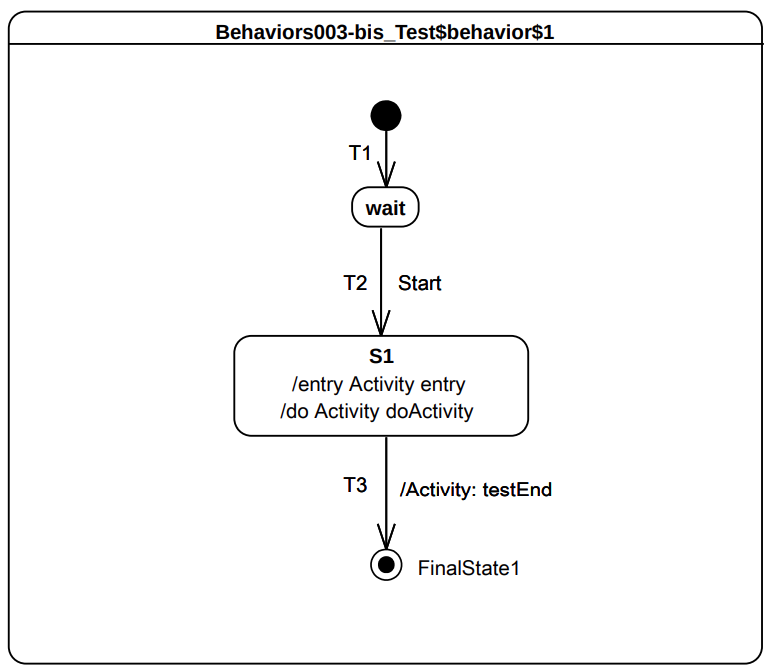
\includegraphics[width=0.6\textwidth]{figures/pssm-003b-sm.png}
    \caption{State Machine Diagram of Target component -- Behavior 003-B~\cite{pssm} test case.}
    \label{fig:pssm-003b-sm}
\end{figure}

The doActivity is shown in \autoref{fig:pssm-003b-do}. It begins its execution by taking a reference of \emph{this} (which is the State Machine's context) and duplicates the value using a \emph{fork} node. The separate branches go to two trace calls -- the first one traces \verb|S1(doActivityPartI)|, while the second one traces \verb|S1(doActivityPartII)|. Since there is an \emph{AcceptEventNode} between the two trace calls, the activity must receive a \emph{Continue} signal to execute the second trace call, finish execution and thus let the statechart reach its final state.

\begin{figure}
    \centering
    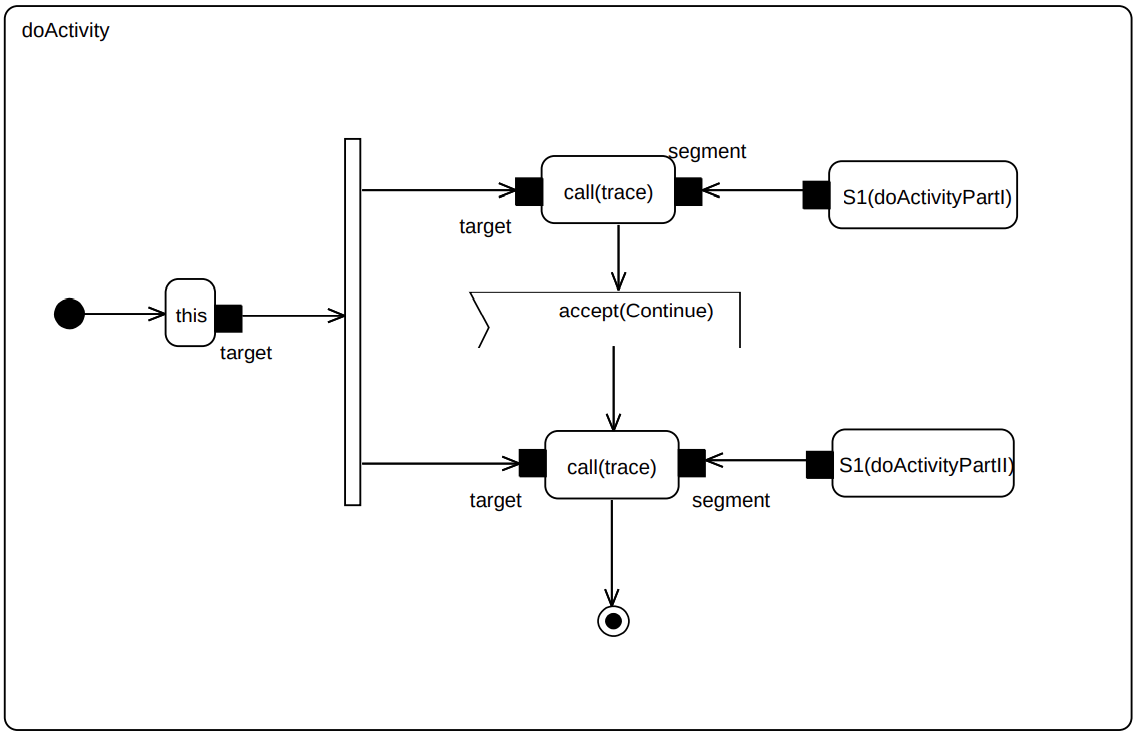
\includegraphics[width=0.8\textwidth]{figures/pssm-003b-do.png}
    \caption{Activity Diagram of S1's doActivity -- Behavior 003-B~\cite{pssm} test case.}
    \label{fig:pssm-003b-do}
\end{figure}

\subsection{Expected Trace}

The PSSM specification lists a single valid execution trace for this model:

\begin{itemize}
    \item \verb|S1(entry)|
    \item \verb|S1(doActivityPartI)|
    \item \verb|S1(doActivityPartII)|
\end{itemize}

The specification also provides the RTC steps during execution, which is shown in \autoref{tab:behavior_003b_rtc}. First, it fires transition \emph{T1} and enters state \emph{wait} as part of the \emph{initial RTC step}. Afterwards, a \emph{completion event} is generated for state \emph{wait}, as it does not have an entry behavior. Since there is no \emph{completion transition} from \emph{wait}, this event is discarded. Given, that the \emph{Start} signal is in the event pool, it triggers transition \emph{T2}. This transition takes the State Machine into state \emph{S1}, which asynchronously starts its doActivity Behavior. Afterward, the State Machine receives a \emph{Continue} signal, which is dispatched to the doActivity, enabling it to finish execution and let \emph{S1} generate a \emph{completion event}. Since S1 has a \emph{completion transition}, it fires, taking the State Machine into its final state, and sending a \emph{testEnd} signal, thus successfully completing the test.

\begin{table}[htbp]
\centering
\begin{tabular}{|l||l|l|l|}
\hline
\textbf{Step} & \textbf{Event pool} & \textbf{State Machine configuration} & \textbf{Fired transitions(s)} \\ \hline\hline
1    & {[}{]}              & {[}{]} - initial RTC step   & {[}T1{]}             \\ \hline
2    & {[}Start, \textbf{CE(wait)}{]} & {[}wait{]}                    & {[}{]}               \\ \hline
3    & {[}\textbf{Start}{]}         & {[}wait{]}                    & {[}T2{]}             \\ \hline
4    & {[}\textbf{Continue}{]}         & {[}S1{]}                    & {[}{]} -- doActivity RTC             \\ \hline
5    & {[}\textbf{CE(S1)}{]}         & {[}S1{]}                    & {[}T3{]}             \\ \hline
\end{tabular}
\caption{The run-to-completion steps for an execution of the Behavior 003-B~\cite{pssm} test case.}
\label{tab:behavior_003b_rtc}
\end{table}

\subsection{Deadlock of Test Model}\label{ssec:deadlock}

Upon closer examination of the PSSM semantics and the test case, we found that in certain situations the model can enter a deadlock\footnote{A state in which the State Machine does not have any more legal steps.} state before reaching its final state, which is not specified as a valid trace by the PSSM standard. The trace of that execution would look like the following:

\begin{itemize}
    \item \verb|S1(entry)|
    \item \verb|S1(doActivityPartI)|
    \item \textbf{(deadlock, final state not reached)}
\end{itemize}

The RTC steps for this trace are shown in \autoref{tab:behavior_003b_deadlock_rtc}. The beginning steps are the same up to the point of entering state \emph{S1}. Given the concurrent nature of doActivities, it is possible, that S1's doActivity does not reach its \emph{AcceptEventAction}, and thus does not register any \verb|EventAccepter| for the \emph{Continue} signal before the \emph{event dispatch} begins. In this case, since there are \textit{no} event accepters for the \textit{Continue} signal, it is \emph{discarded}. After this point, the doActivity will reach its trace action and \textit{AcceptEventNode}, thus registering a new event accepter for the \textit{Continue} signal. Since doActivities are only considered completed when they \emph{do not} have any event accepters registered and have no more actions to execute, the doActivity remains active, which prevents \textit{S1} from generating a completion event, thus the State Machine may never fire \textit{T3}. After this point, the State Machine has no more steps to take, thus the test case will never complete.

\begin{table}[htbp]
\centering
\begin{tabular}{|l||l|l|l|}
\hline
\textbf{Step} & \textbf{Event pool} & \textbf{State Machine configuration} & \textbf{Fired transitions(s)} \\ \hline\hline
1    & {[}{]}              & {[}{]} - Initial RTC step   & {[}T1{]}             \\ \hline
2    & {[}Start, \textbf{CE(wait)}{]} & {[}wait{]}                    & {[}{]}               \\ \hline
3    & {[}\textbf{Start}{]}         & {[}wait{]}                    & {[}T2{]}             \\ \hline
4    & {[}\textbf{Continue}{]}         & {[}S1{]}                    & {[}{]}             \\ \hline
\end{tabular}
\caption{The run-to-completion steps for a deadlocked execution of the Behavior 003-B~\cite{pssm} test case.}
\label{tab:behavior_003b_deadlock_rtc}
\end{table}

\subsection{Conclusion}

The possible deadlock of this model was found by the \textit{exhaustive} simulator which demonstrates the value of this approach and the usability of the simulator itself. The simulator traversed every possible execution of the model, aggregated the executions, and presented them graphically.

\autoref{fig:behavior003b-actual} shows the generated execution traces by tracking only the Target log variables: $V_{T_1} = \{ v_{\mathrm{log_{target}}}, v_{\mathrm{log_{doActivity}}} \}$. The simulator also found the execution trace of reaching the \emph{deadlock} state. This trace is refined in \autoref{fig:behavior003b-dispatcher}, which shows the generated execution traces by tracking the Target logs and the Dispatcher logs as well: $V_{T_2} = V_{T_1} \cup \{ v_{\mathrm{log_{dispatcher}}} \}$.

Note, that \autoref{fig:behavior003b-actual} and \autoref{fig:behavior003b-dispatcher} show the same execution traces, only with different granularity. In \autoref{fig:behavior003b-actual}, only the PSSM-level trace statements (modeled as Gamma log statements) are shown which also serves as an example for the back-annotation of the low-level simulation to the high-level. In \autoref{fig:behavior003b-dispatcher}, the execution traces contain more details demonstrating the customizable set of tracked variables.

\begin{figure}
\centering
\includesvg[inkscapelatex=false, height=200pt, keepaspectratio]{figures/behavior003b-actual.svg}
\caption{The actual execution traces of Behavior 003-B~\cite{pssm}, found by our approach with tracking variables $V_{T_1}$. The expected execution trace defined by PSSM is colored green, while the execution trace reaching a deadlocked state (discussed in \autoref{ssec:deadlock}) is colored red~\cite{tdk}.}
\label{fig:behavior003b-actual}
\end{figure}

\begin{figure}
\centering
\includesvg[inkscapelatex=false, width=\textwidth, keepaspectratio]{figures/behavior003b-dispatcher.svg}
\caption{The actual execution traces of Behavior 003-B~\cite{pssm}, found by our approach with tracking variables $V_{T_2}$. The nodes representing dispatcher interactions (discussed in \cite{tdk}) are filled with gray, in their label D denotes the dispatcher, SC denotes the statechart, and A denotes the activity. The deadlocked execution traces (discussed in \autoref{ssec:deadlock}) are colored red. The red nodes show the reasons for the deadlocks, i.e. that the statechart sends the ignore message to the dispatcher before the subscription of the activity~\cite{tdk}.}
\label{fig:behavior003b-dispatcher}
\end{figure}

\chapter{Conclusion} \label{conclusion}

For the design of more complex systems, more complex modeling languages with higher abstraction levels are needed. Due to the increasing complexity, the need for \textit{systematic} approaches is growing, too. In the case of behavioral models, this means the \textit{precise} simulation of models, i.e., revealing every possible decision point during the execution, derived from the complex semantics.

In this thesis, I gave an overview of formal methods, formal models, and model simulation. For the modeling of component-based reactive systems, I presented modeling languages with different abstraction levels. These languages have precise formal semantics, as well as open-source tools supporting them.

I defined the requirements on a step-by-step controllable simulation framework for such models and presented my algorithm to make internal non-determinism external, which I implemented as an extension of the Gamma Statechart Composition Framework. I designed a simulation framework based on existing model checking infrastructure and implemented it as an extension of the Theta Model Checking Framework.

Finally, I presented the usage of my work through a case study about the validation of the UML PSSM standard using the exhaustive simulator to generate every possible execution of state machine models.

\section{Future Work} \label{future-work}

For future improvements of the simulator, I have collected a set of requirements that could improve on existing functionalities or extend the tool with useful features.

The simulator should back-annotate every low-level (XSTS) state change to the high-level (statechart) -- instead of back-annotating only the log statements. The simulator should support the tracking of general expressions over the variables -- instead of supporting only individual variables. The simulator should be able to replay execution traces -- supporting the saving, reloading, and replaying of simulation states/execution traces.

The user interface of the simulator could be improved, too. The simulator should be integrated into common IDEs (e.g., Eclipse or Visual Studio Code over Language Server Protocol) -- making its usage more convenient and supporting widely-used debugging use cases, e.g., breakpoints.


% Acknowledgements
%~~~~~~~~~~~~~~~~~~~~~~~~~~~~~~~~~~~~~~~~~~~~~~~~~~~~~~~~~~~~~~~~~~~~~~~~~~~~~~~~~~~~~~
%----------------------------------------------------------------------------
\selecthungarian
\chapter*{Köszönetnyilvánítás}\addcontentsline{toc}{chapter}{Köszönetnyilvánítás}
%----------------------------------------------------------------------------

Számomra ez a diplomaterv a maga módján túlmutat önmagán: nemcsak a mesterképzésem lezárásának tekintem, hanem egyúttal egy mérföldkőnek is, amely az eddigi, tanulmányaim köré szerveződő életszakaszomat választja el az ezután következőtől. Éppen ezért, kissé talán rendhagyó módon, szeretném megragadni a lehetőséget, hogy itt is köszönetet mondjak mindazoknak, akik segítettek az idáig vezető úton.

Köszönöm \textit{szüleimnek}, hogy lehetővé tették, hogy az elmúlt öt és fél évben az egyetemi tanulmányaimra koncentrálhassak, \textit{középiskolai tanáraimnak}, hogy biztos alapokat adtak ehhez, valamint bátyáimnak, \textit{Bencének} és \textit{Zolinak}, hogy a legkülönbözőbb kérdéseimet is mindig igyekeztek megválaszolni. Köszönöm évfolyamtársaimnak, barátaimnak, hogy együtt jártuk végig ezt az utat: \textit{Benedek, Dani, Domonkos, Jonatán, Józsi, Ricsi} – a segítségetek nélkül sokkal göröngyösebb lett volna.

Köszönöm a \textit{Kritikus Rendszerek Kutatócsoport} minden tagjának, aki bármiben segített az itt töltött éveim során, különösen \textit{Majzik Istvánnak}, hogy konzulensként segített a kezdetekben, \textit{Micskei Zoltánnak}, hogy végig rajtam tartotta a szemét és egyengette az utamat, \textit{Elekes Mártonnak} és \textit{Graics Bencének}, hogy energiát nem kímélve konzultálták a TDK dolgozatunkat, valamint \textit{Vörös Andrásnak}, hogy mindig volt egy biztató szava és hasznos észrevétele.

Külön köszönöm konzulensemnek, \textit{Molnár Vincének}, hogy ennyi éven keresztül végigkísérte az utamat: kezdve a középiskolai szakköröktől, ahol megismertette velem a programozást, a szakdolgozatomon és a TDK dolgozatunkon keresztül egészen ennek a diplomatervnek a konzultálásáig. Lehetetlen lenne felsorolni, mennyit tanultam tőle mind szakmailag, mind emberileg, és mindig hálás leszek a feltétel nélküli támogatásáért, amit akkor nyújtott, amikor a legnagyobb szükségem volt rá.

Úgy alakult, hogy életem más területei tartogattak néhány nehézséget az elmúlt időszakban, amikor ez a diplomaterv is készült.
Köszönöm barátaimnak, hogy ezekben az időkben is mellettem álltak és támogattak: \textit{Ági, Anna, Bence, Dani, Dórik, Gergő, Hanga, Körte, Levi, Máté, Mosi, Nándi, Pali, Réka, Sajt, Szander, Viktorok, Virág, Zsófi, Zsuzsi} – nélkületek minden sokkal nehezebb lett volna.

\epigraph{\textit{– Vége? – kérdezte Róbert Gida. \\
– Ennek. De van más mesém.}}{A. A. Milne: \textit{Micimackó}}

\selectenglish



% List of Figures, Tables
%~~~~~~~~~~~~~~~~~~~~~~~~~~~~~~~~~~~~~~~~~~~~~~~~~~~~~~~~~~~~~~~~~~~~~~~~~~~~~~~~~~~~~~
%\listoffigures\addcontentsline{toc}{chapter}{\listfigurename}
%\listoftables\addcontentsline{toc}{chapter}{\listtablename}
%\listofalgorithms\addcontentsline{toc}{chapter}{\listalgorithmcfname}


% Bibliography
%~~~~~~~~~~~~~~~~~~~~~~~~~~~~~~~~~~~~~~~~~~~~~~~~~~~~~~~~~~~~~~~~~~~~~~~~~~~~~~~~~~~~~~
% Source: https://tex.stackexchange.com/questions/8458/making-the-bibliography-appear-in-the-table-of-contents
\cleardoublepage
\phantomsection

\addcontentsline{toc}{chapter}{\bibname}
\bibliography{bib/mybib}



% Appendix
%~~~~~~~~~~~~~~~~~~~~~~~~~~~~~~~~~~~~~~~~~~~~~~~~~~~~~~~~~~~~~~~~~~~~~~~~~~~~~~~~~~~~~~
%\include{content/appendices}

%\label{page:last}
\end{document}
